\PassOptionsToPackage{svgnames}{xcolor}
\documentclass[12pt]{article}



\usepackage[margin=0.1in]{geometry}  
\usepackage{graphicx}             
\usepackage{amsmath}              
\usepackage{amsfonts}              
\usepackage{framed}               
\usepackage{amssymb}
\usepackage{array}
\usepackage{amsthm}
\usepackage{multirow}
\usepackage[nottoc]{tocbibind}
\usepackage{bm}
\usepackage{enumitem}
\usepackage{tikz}
\usepackage{pdfpages}
\usepackage{titlesec}
\titlespacing*{\section}{0pt}{0.5\baselineskip}{0.5\baselineskip}
\newcolumntype{C}[1]{>{\centering\let\newline\\\arraybackslash\hspace{0pt}}m{#1}}


  \newcommand\norm[1]{\left\lVert#1\right\rVert}
\setlength{\parindent}{0cm}
\setlength{\parskip}{0em}
\newcommand{\Lim}[1]{\raisebox{0.5ex}{\scalebox{0.8}{$\displaystyle \lim_{#1}\;$}}}
\newtheorem{definition}{Definition}[section]
\newtheorem{theorem}{Theorem}[section]
\newtheorem{notation}{Notation}[section]
\theoremstyle{definition}
\DeclareMathOperator{\arcsec}{arcsec}
\DeclareMathOperator{\arccot}{arccot}
\DeclareMathOperator{\arccsc}{arccsc}
\DeclareMathOperator{\spn}{Span}
\setcounter{tocdepth}{1}
\begin{document}

\title{Revision notes - CS2106}
\author{Ma Hongqiang}
\maketitle
\tableofcontents


\twocolumn
\section{Introduction to OS}
\subsection{Operating System Basic Concepts}
\begin{definition}[No OS]
\hfill\\\normalfont There is no OS for the first computer where programmes \textit{directly} interact with hardware, and reprogramming is done through changing the \textbf{physical configuration} of the hardware.\\
\textbf{Advantage}:
\begin{itemize}
  \item Minimal overhead
\end{itemize}
\textbf{Disadvantage}:
\begin{itemize}
  \item Programmes are not portable
  \item Utilisation of Computing resource is low
\end{itemize}
\end{definition}
\begin{definition}[Batch OS]
\hfill\\\normalfont Batch OS breaks down the workflow to Input, Compute and Output, which allows pipelining to occur.\\
Programmes can be \textit{submitted in batch} to be \textit{executed one at a time}. \\
However, batch processing is still inefficient since the CPU will be idle when I/O. One solution is \textbf{multiprogramming}, where multiple jobs are loaded and other jobs are to be ran when I/O needs to be done.
\end{definition}
\begin{definition}[Time-sharing OS]
\hfill\\\normalfont Time-sharing OS allows multiple users to interact with machine using terminals(\textbf{teletypes}). It provides user job scheduling which gives \textit{illusion} of concurrency. \\
\begin{figure}[h]
\centering
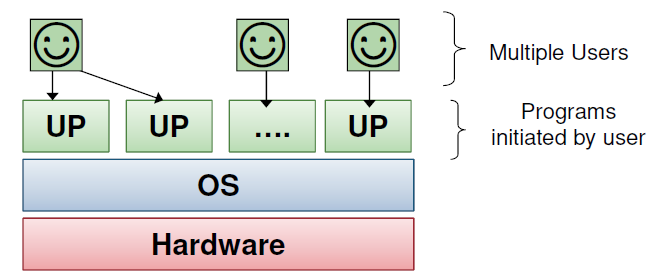
\includegraphics[width = 0.4\textwidth]{1_3.png}
\end{figure}
It provides CPU time, memory and storage management; essentially, it provides \textbf{virtualisation of hardware}, where each program executes as if it has all the resources to itself.
\end{definition}
\begin{definition}[Personal OS]
\hfill\\\normalfont Personal OS is dedicated to machine that dedicates to one user, which is not time shared.\\
There are several models:
\begin{enumerate}
  \item Windows Model:
  \begin{itemize}
    \item Single user at a time but possibly more than 1 user can access
    \item dedicated machine
  \end{itemize}
  \item Unix Model:
  \begin{itemize}
    \item One user at the workstation but others can access remotely
    \item General time sharing model
  \end{itemize}
\end{enumerate}
\end{definition}
\subsection{Motivation of OS}
There are three main motivations:
\begin{enumerate}
  \item Abstraction over the hardware, which has
  \begin{itemize}
    \item \textit{Different} capacity
    \item \textit{Different} capability, but
    \item Well-defined and \textit{common} functionality
  \end{itemize}
  so that low level details can be hidden and only high level functionality is presented. It provides efficiency and portability.
  \item Resource Allocator, which 
  \begin{itemize}
    \item Manages all resources such as CPU, Memory, I/O devices
    \item Arbitrate potentially conflicting requests, for efficient and fair resource use
  \end{itemize}
  \item Control Program, which controls execution of programmes so as to 
  \begin{itemize}
    \item Prevent errors and improper use of the computer, accidentally or maliciously
    \item Provide security and protection
  \end{itemize}
\end{enumerate}
\subsection{OS Structure}
Operating System structure needs to impart flexibility, robustness and maintainability. Generally, the high level view of OS is that
\begin{itemize}
  \item Operating system is essentially a \textbf{software}, which has the privilege to run in \textbf{kernel mode}, i.e., has complete access to all hardware resources
  \item Other software executes only in \textbf{user mode}, with limited access to hardware resources
\end{itemize}
However, one must realise the user programme can interact with hardware through OS or else. Following diagram gives you an overview:
\begin{figure}[h]
\centering
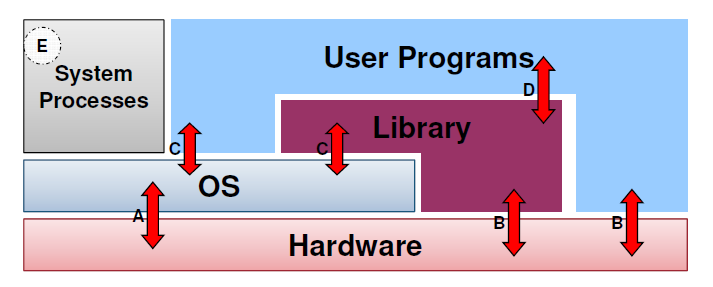
\includegraphics[width = 0.4\textwidth]{1_5.png}
\end{figure}
\begin{itemize}
  \item $A$: OS executing machine instructions
  \item $B$: normal machine instructions executed
  \item $C$: calling OS using \textbf{system call interface}, e.g. \texttt{fopen()}
  \item $D$: user program calls library code, e.g. \texttt{pow()}
  \item $E$: system processes, which provide \textit{high} level services, and is usually part of the OS
\end{itemize}

In terms of functionality, OS is known as the \textbf{kernel}, which is a programme providing special features like:
\begin{itemize}
  \item Deals with hardware issues
  \item Provides system call interface
  \item Special code for interrupt handlers, device drivers
\end{itemize}
However, kernel code has to be different than normal program as
\begin{itemize}
  \item No use of system call in kernel code
  \item Cannot use normal libraries
  \item There is no normal I/O
\end{itemize}
Currently, the common code organisation consists of
\begin{itemize}
  \item Machine independent high level language(HLL)
  \item Machine dependent HLL
  \item Machine dependent assembly code
\end{itemize}
In terms of implementation, there are few ways to structure an OS, most notably monolithic or microkernel.
\begin{definition}[Monolithic OS]
\hfill\\\normalfont Monolithic OS kernel has the defining characteristics of
\begin{itemize}
  \item One \textbf{big} special program, where various services and compopnents are integral part.
\end{itemize}
\begin{figure}[h]
\centering
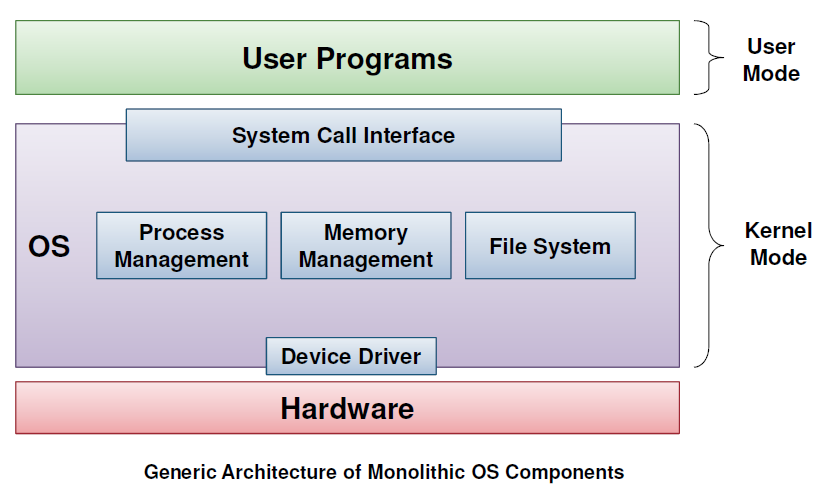
\includegraphics[width = 0.4\textwidth]{1_6.png}
\end{figure}
Monolithic kernel has the advantage of
\begin{itemize}
  \item Well understood
  \item Good performance
\end{itemize}
It has the disadvantage of
\begin{itemize}
  \item Highly coupled components
  \item Usually devolved into very complicated internal structure
\end{itemize}
\end{definition}
\begin{definition}[Microkernel OS]
\hfill\\\normalfont Microkernel OS kernel has the defining characteristics of 
\begin{itemize}
  \item Very small and clean
  \item Only provides basic and essential facilities:
  \begin{itemize}
    \item Inter-Process Communication(IPC)
    \item Address space management
    \item Thread management
    \item etc
  \end{itemize}
\end{itemize}
Higher level services like Process Management are
\begin{itemize}
  \item Built \textit{on top of} the basic facilities
  \item Run as server process \textbf{outside} of the OS
  \item Use IPC to communicate
\end{itemize}
\begin{figure}[h]
\centering
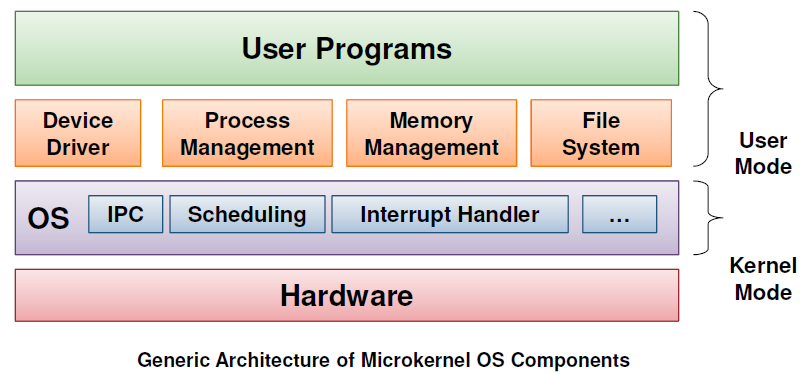
\includegraphics[width = 0.4\textwidth]{1_7.png}
\end{figure}
Microkernel OS has the advantage of
\begin{itemize}
  \item Kernel is generally more robust and more extendible
  \item Better isolation and protection between kernel and high level services
\end{itemize}
It has the disadvantage of
\begin{itemize}
  \item Lower performance
\end{itemize}
\end{definition}
Other OS structure include layered systems, client-server model etc.
\begin{definition}[Virtual Machine]
\hfill\\\normalfont Virtual Machine, or \textbf{hypervisor} is a software emulation(virtualisation) of hardware.
\end{definition}
Normal(primitive) operating systems can then run on top of the virtual machine.\\
There are two type of hypervisor:
\begin{figure}[h]
\centering
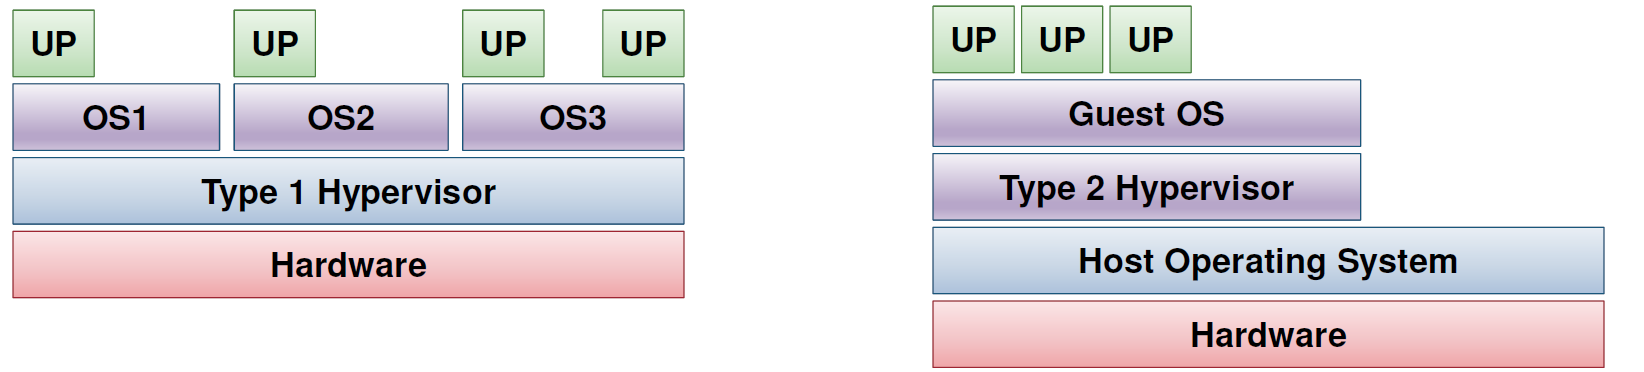
\includegraphics[width = 0.4\textwidth]{1_8.png}
\caption{Type 1 Hypervisor(left) and Type 2 Hypervisor(right)}
\end{figure}
\begin{itemize}
  \item Type 1: provides individual virtual machines to guest OSes
  \item Type 2: runs in host OS and only guest OS runs in Virtual Machine
\end{itemize}

\section{Process Abstraction}
\begin{definition}[Process]
\hfill\\\normalfont \textbf{Process}/task/job is a dynamic abstraction for executing program, where information required to describe a running program is contained. The information includes three components:
\begin{itemize}
  \item Memory context
  \item Hardware context
  \item OS context
\end{itemize}
\end{definition}
\subsection{Memory Context}
From \texttt{CS2100}, we know that memory contains a 
\begin{itemize}
  \item \textbf{Text} section, to store instructions
  \item \textbf{Data} section, to store global variables
\end{itemize}
However, these two sections are unable to handle function call.
\begin{definition}[Caller, Callee]
\hfill\\\normalfont When \texttt{f()} calls \texttt{g()}, \texttt{f()} is the \textbf{caller} whereas \texttt{g()} is the \textbf{callee}.
\end{definition}
To handle function call, we require a new section called \textbf{Stack}.
\begin{definition}[Stack]
\hfill\\\normalfont Stack is used to store information about function invocation. The information of a function invocation is described by a \textbf{stack frame}.\\
Since stack can be of variable size, the top of the stack region is logically indicated by \textbf{stack pointer}. Stack pointer usually is stored in a specialised register in the CPU.
\begin{figure}[h]
\centering
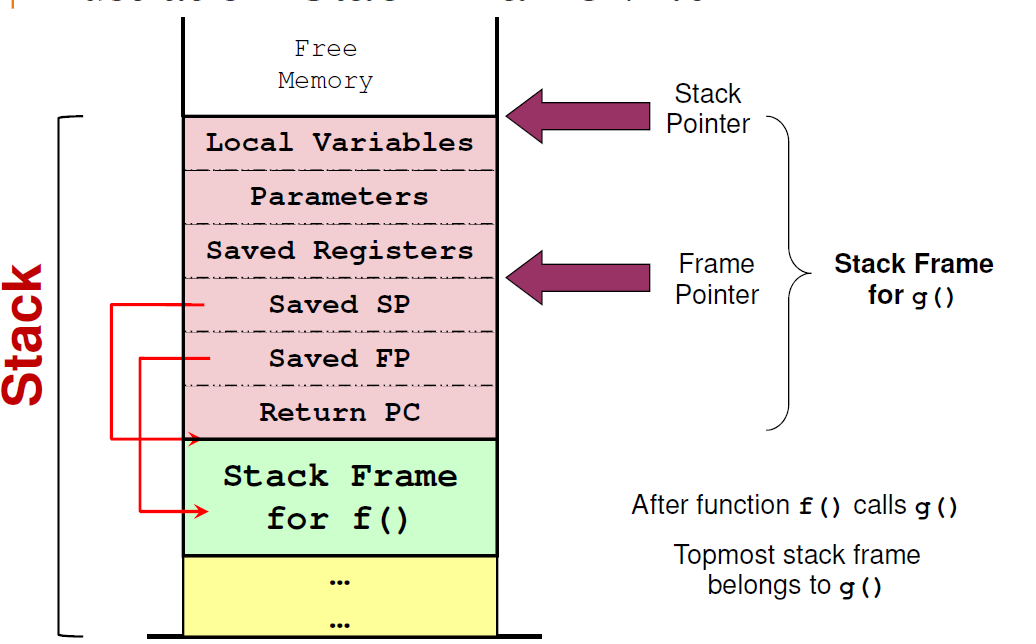
\includegraphics[width=0.4\textwidth]{2_1.png}
\end{figure}
Usually, a stack farme contains the following items
\begin{itemize}
  \item Local variables
  \item Function parameters
  \item Saved Registers
  \item Saved Stack Pointer
  \item Saved Frame Pointer
  \item Return Programme Counter(PC)
\end{itemize}
\end{definition}
\begin{definition}[Frame Pointer]
\hfill\\\normalfont Stack pointer can move during function execution. For example, the stack pointer can shift during a control statement \texttt{if}.\\
To facilitate the access of various stack frame items, a \textbf{frame pointer} can be used, which points to a \textbf{fixed location} in a stack frame. Other items can be accessed as a displacement from the frame pointer.
\end{definition}
\begin{theorem}[Stack Frame Setup/Teardown]
\hfill\\\normalfont On executing function call,
\begin{enumerate}
  \item \textbf{Caller}: Pass arguments with registers and/or stack
  \item \textbf{Caller}: Save Return PC on stack
  \item \textbf{Transfer control from caller to callee}
  \item \textbf{Callee}: Save registers used by callee. Save old FP, SP.
  \item \textbf{Callee}: Allocate space for local variables of callee on stack
  \item \textbf{Callee}: Adjust SP to point to new stack top
\end{enumerate}
On returning from function call:
\begin{enumerate}
  \item \textbf{Callee}: Restore saved registers, FP, SP
  \item \textbf{Transfer control from callee to caller using saved PC}
  \item \textbf{Caller}: Continues execution in caller
\end{enumerate}
\end{theorem}
\textbf{Remark}: There is no universal way of doing function call. The above is just a example.
\begin{definition}[Heap Memory Region]
\hfill\\\normalfont Heap Memory Region is a memory region that supports \textbf{dynamically allocated memory}, which is acquisition of memory space during \textbf{execution time}.
\end{definition}
Heap memory is trickier to manage due to its nature:
\begin{itemize}
  \item Variable Size
  \item Variable Allocation/Deallocation Timing
\end{itemize}
Its nature will create scenario where heap memory are allocated and deallocated in a way that creates holes in memory.\\

The actual memory context contains the four regions described above, namely text, data, heap and stack.
\begin{figure}[h]
\centering
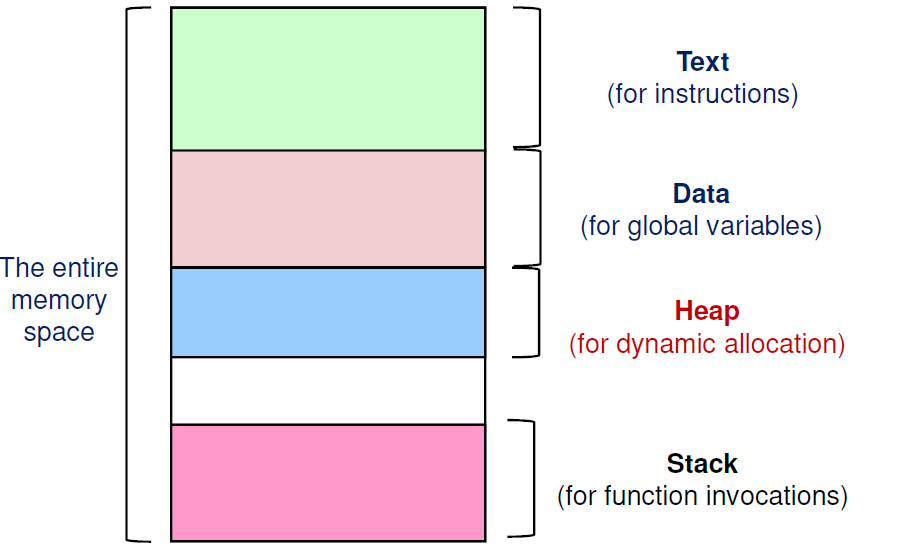
\includegraphics[width=0.4\textwidth]{2_2.png}
\end{figure}
\subsection{Hardware Context}
In correspondence to the memory context, the hardware context contains
\begin{itemize}
  \item General Purpose Registers
  \item Program Counter
  \item Stack Pointer
  \item Stack Frame Pointer
\end{itemize}
\subsection{OS Context}
\begin{definition}[Process ID]
\hfill\\\normalfont Process ID is to distinguish processes from each other, and it is unique among processes.
\end{definition}
Apart from Process ID, we also need a process state, to describe the state of the process, e.g. running or not running.
\begin{definition}[Generic 5-state Process Model]
\begin{figure}[h]
\centering
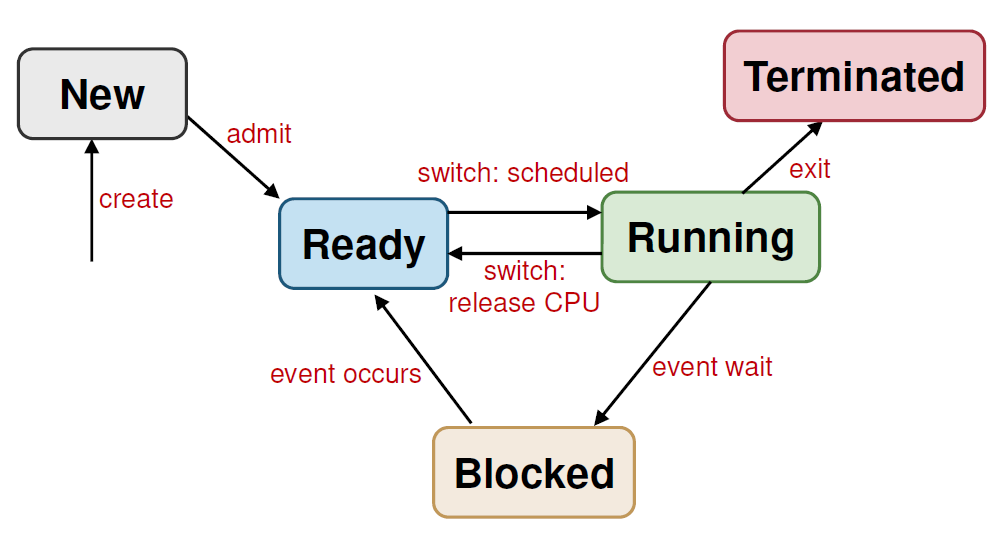
\includegraphics[width=0.4\textwidth]{2_3.png}
\end{figure}
\hfill\\\normalfont The Generic 5-state Process Model contains 5 states:
\begin{enumerate}
  \item New
  \begin{itemize}
    \item New process created
    \item May still be under initialisation, therefore \textit{not yet} ready
  \end{itemize}
  \item Ready
  \begin{itemize}
    \item Process is waiting to run
  \end{itemize}
  \item Running
  \begin{itemize}
    \item Process is being executed on CPU
  \end{itemize}
  \item Blocked
  \begin{itemize}
    \item Process waiting/sleeping for event
    \item Cannot execute until event is available
  \end{itemize}
  \item Terminated
  \begin{itemize}
    \item Process has finished execution, may require OS cleanup
  \end{itemize}
\end{enumerate}
There are also different state transitions,
\begin{enumerate}
  \item Create(NIL $\to$ New): new process is created
  \item Admit(New $\to$ Ready): process ready to be scheduled for running
  \item Switch(Ready $\to$ Running): process selected to run
  \item Switch(Running $\to$ Ready): process gives up CPU voluntarily or \textbf{pre-empted} by scheduler
  \item Event Wait(Running $\to$ Blocked): Process requests event/resource/service(system call, I/O, etc.) which is not available, or in progress
  \item Event Occurs(Blocked $\to$ Ready): Event occurs, which means process can continue
\end{enumerate}
\end{definition} 
In CS2106, we admit a simplified view on CPU: there is only 1 CPU, which means there is
\begin{itemize}
  \item $\leq 1$ process in running state
  \item conceptually 1 transition at a time
\end{itemize}
As there may be multiple processes ready for run, or awaiting resources, we use a queuing model to describe the 5-state transition.
\begin{figure}[h]
\centering
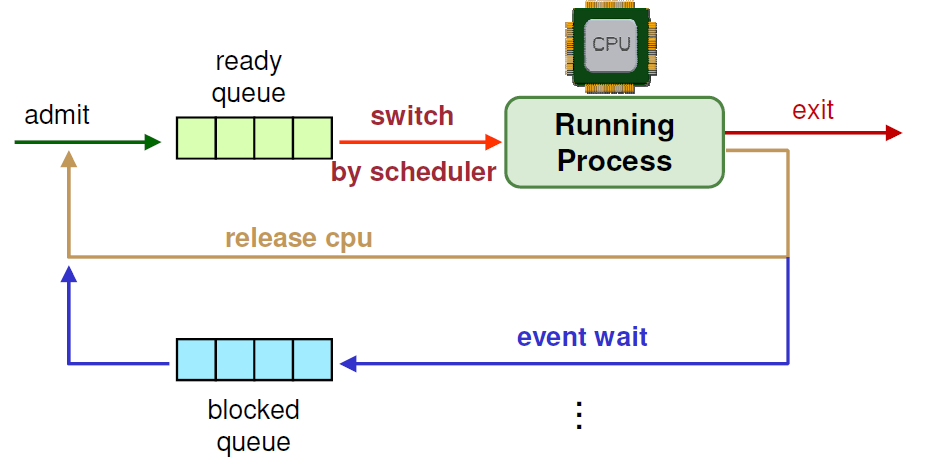
\includegraphics[width=0.4\textwidth]{2_4.png}
\end{figure}
Note, here the ready queue and the blocked queue should be viewed as \textbf{set}, not queue.\\

Up to this point, the OS context contains
\begin{itemize}
  \item Process ID,
  \item Process State
\end{itemize}
\subsection{Process Control Block}
The entire execution context for a process is stored in \textbf{Process Control Block}, maintained by the kernel. The process control block(PCB) contains memory, hardware and process context.\\
\begin{figure}[h]
\centering
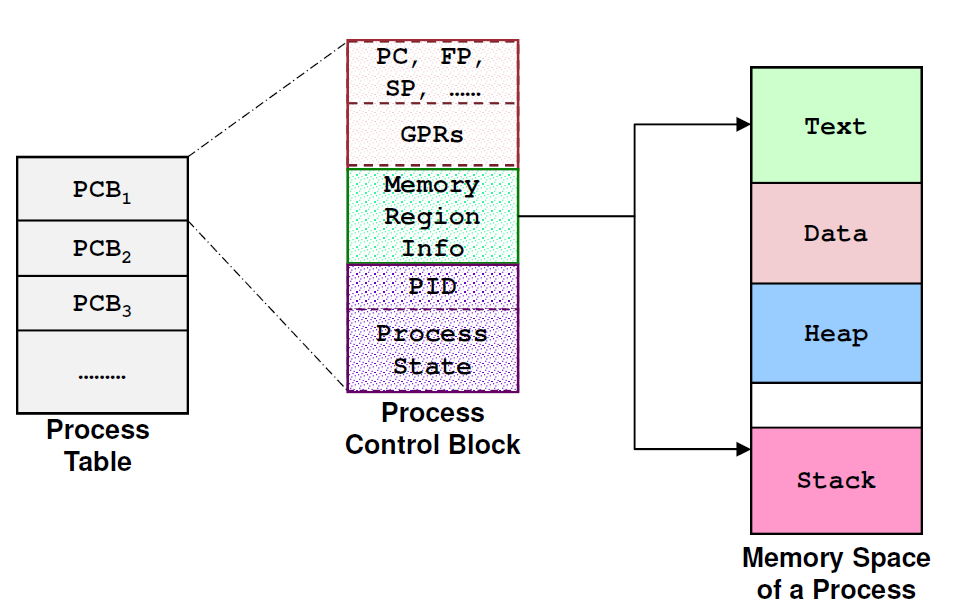
\includegraphics[width=0.4\textwidth]{2_5.png}
\end{figure}
 A process Table contains process control blocks of all processes.
\subsection{System Calls}
System calls are Application Program Interface(API) to OS, which provides ways of calling facilities/services in kernel.\\It is \textbf{not} the same as normal function call since it has to change from user mode to kernel mode.\\
Different OS will then have different APIs, for example:
\begin{itemize}
  \item UNIX variant: POSIX standard, which has small number($\approx 100$) of calls
  \item Windows family: Win API, which has $\approx 1000$ number of calls
\end{itemize}
In \texttt{C}, system calls can be invoked almost directly, but the function we call is not the actual system call, as we need to have a setup before the actual call. Therefore, the function we call can be
\begin{itemize}
  \item Function Wrapper, which is the same name and has the same parameters and the actual call, but handles the setup for caller. \\One example is \texttt{getpid()}.
  \item Function Adapter, which is a library function with less number of parameters and possibly more flexible parameter values.\\One example is \texttt{printf()}, which uses \texttt{write()} system call in its implementation.
\end{itemize}
\begin{theorem}[General System Call Mechanism]
\hfill\\\normalfont Generally, system call by user programme is handled in this manner:
\begin{enumerate}
  \item User program invokes the library call
  \item Library call, usually in assembly code, places the \textbf{system call number} is a designated location, e.g., a register.
  \item Library call executes a special instruction to switch from user mode to kernel mode. The special instruction is commonly known as \textbf{TRAP}. 
  \item Now, in kernel mode, the appropriate system call handler is determined, by using the system call number as an index. \\This step is usually handled by a \textbf{dispatcher}.
  \item System call handler is executed, carrying out the actual request.
  \item System call handler ended, and control is returned to the library call. \\We switch from kernel mode back to user mode.
  \item Library call return to the user program, via normal function return mechanism.
\end{enumerate}
\end{theorem}
\subsection{Exception and Interrupt}
\subsubsection{Exception}
Executing a \textbf{machine level instruction} can cause exception. For example, arithmetic error, or memory accessing errors are two common types of exceptions.\\
Exception is \textbf{synchronous}, in the sense that it occurs due to the program execution.\\
The effect of exception is 
\begin{itemize}
  \item Have to execute a \textbf{exception handler}. This exception handler is similar to a \textbf{forced function call}.
\end{itemize}
\subsubsection{Interrupt}
\textit{External} events can interrupt the execution of a program. The cause of interrupt is usually hardware related, for example \texttt{Ctrl + C}.\\
Interrupt, unlike exception, is therefore \textbf{asynchronous}, as it occurs independent of program execution.\\
The effect of interrupt is
\begin{itemize}
  \item Program execution is suspended, by executing an \textbf{interrupt handler}.
\end{itemize}
For the exception/interrupt handler, it is transferred control automatically to when an exception/interrupt occurs. Inside the handler, it performs the following routine
\begin{enumerate}
  \item Save Register/CPU state
  \item Perform the handler routine
  \item Restore Register/CPU
  \item Return from interrupt
\end{enumerate}
After the return from handler routine, program execution will resume, and the programme \textit{may} behave as if nothing happened.

\section{Process Abstraction in UNIX}
\subsection{Identification}
A process in UNIX is uniquely identified by Process ID(PID), which is integer-valued.
\subsection{Information}
A process will keep track of the information of
\begin{itemize}
  \item \textbf{Proecss State}: Running, Sleeping, Stopped, Zombie
  \item \textbf{Parent PID}: PID of the parent process
  \item \textbf{Cumulative CPU time}: Total Amount of CPU time used so far
  \item etc
\end{itemize}
Unix command \texttt{ps} can extract the process information
\subsection{Process Creation}
\texttt{fork()} is the main way to create a new process. It returns
\begin{itemize}
  \item \texttt{PID} of the newly created process for parent process, or
  \item $0$ for child process
\end{itemize}
The behaviour of \texttt{fork()} is to create a new process called \textbf{child process}, which is a \textbf{duplicate} of the current executable image. The data in child is a \textbf{copy} of the parent, thus not shared. The \textit{only} difference between the parent and child process are
\begin{itemize}
\item Process ID(PID)
\item Parent ID(PPID)
\item \texttt{fork()} return value
\end{itemize}
Note, after \texttt{fork()}, both parent and child processes continue executing after \texttt{fork()}. If we want to make parent and child processes to behave differently, we can leverage on the \texttt{fork()} return value.
\subsection{Executing New Programe/Image}
\texttt{fork()} is not useful if you want to execute the original process and another process which is different from the original. Suppose the another process' code is provided as a new executable, then we can use \texttt{exec()} system calls family.\\

Specifically, one can use \texttt{execl()} to \textbf{replace} current executing process image with a new one. This replacement will change 
\begin{itemize}
  \item Code
  \item Memory content
\end{itemize}
but PID and other information will still be \textit{intact}.\\
\texttt{execl} takes the form of \texttt{execl const char *path, const char *arg0,...,const char *argN, NULL)}, where
\begin{itemize}
  \item \texttt{path} is the location of the executable
  \item \texttt{arg0} is the executable name
  \item \texttt{arg1} to \texttt{argN} are vararg command line arguments, corresponding to \texttt{argv[1]} to \texttt{argv[n]}.
  \item The last \texttt{NULL} is used to terminate the vararg array.
\end{itemize}
Therefore, we can combine \texttt{fork()} with \texttt{exec()} to
\begin{itemize}
  \item Spawn off a child process via \texttt{fork()}, which is replaced to the actual task process by invoking \texttt{exec()}.
  \item Parent process remains intact, which can continue to execute.
\end{itemize}
In fact, this way of invoking new processes is common across UNIX. Therefore, to start off, we need a special initial process, namely the \texttt{init} process, which is created in kernel at boot up time with a PID 1. The \texttt{init} process watches for other processes and respawns where needed. Other processes are created by invoking \texttt{fork()} on \texttt{init} or child of \texttt{init}. 
\subsection{Process Termination}
To end execution of process, we can use \texttt{exit(status)}. The status will be returned to the parent process, by which this child process is created.\\
The UNIX convention is to \texttt{exit} with a status $0$ if the termination is normal, and non-zero if the execution is problematic.\\
\textbf{Remark}: This function itself does not return.\\
When \texttt{exit(status)} is executed, \textit{most} system resources used by process are released. However, some basic process resources are \textbf{not releasable}. This includes
\begin{itemize}
\item PID and status, which is required for parent-children synchronisation
\item Process accounting information, e.g., CPU time\
\item Also, process table entry \textit{may be} still needed
\end{itemize}   
As most programs do not have explicit \texttt{exit()} call, return from main function will implicitly calls \texttt{exit()}, and as a result, open files will get flushed automatically, since file descriptors will be released.
\subsection{Parent/Child Synchronisation}
Parent process can wait for child process to terminate, by invoking \texttt{wait(*status)}. This call of \texttt{wait(*status)} will return the PID of the terminated child process. Also, the address where the \texttt{status} pointer points to will be populated with the exit status of the terminated child process.\
The behaviour of \texttt{wait()} is as follows
\begin{itemize}
  \item \texttt{wait()} is blocking: parent process is blocked until at least one child terminates
  \item The call cleans up \textbf{remainder} of the child system resources, which includes
  \begin{itemize}
    \item Those not removed on \texttt{exit()}, and also
    \item Kills zombie process
  \end{itemize}
\end{itemize}
Other variant of \texttt{wait()} includes
\begin{itemize}
  \item \texttt{waitpid()}, which waits for a specific child proecss
  \item \texttt{waitid()}, which waits for any child process to \textbf{change status}
\end{itemize}
Therefore, we can summarise the process interaction in UNIX as follows:
\begin{figure}[h]
\centering
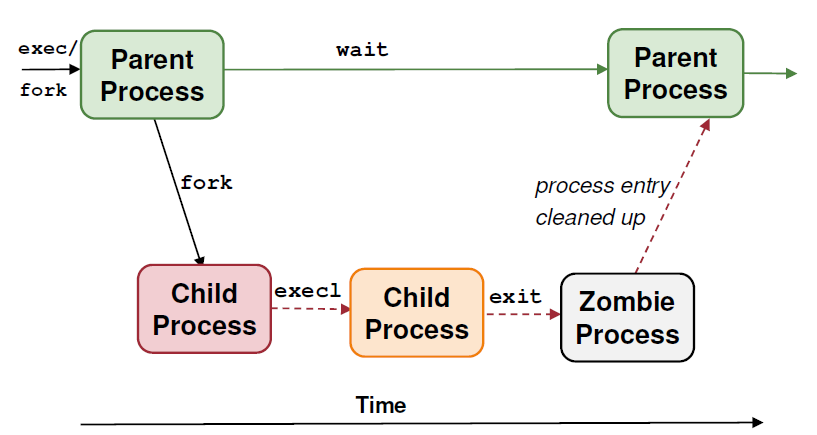
\includegraphics[width=0.4\textwidth]{3_1.png}
\end{figure}
Therefore, one point to note is that, suppose the parent does not \texttt{wait}, the zombie process cannot be cleaned up by the parent. Therefore, to handle this scenario, there are two cases to consider:
\begin{itemize}
  \item[Case 1] Parent process terminates before child process:
  \begin{itemize}
    \item \texttt{init} process becomes "pseudo" parent of child processes
    \item Child termination sends signal to \texttt{init}, which utilises \texttt{wait} to cleanup.
  \end{itemize}
  \item[Case 2] Child process terminates before parent, but parent did not call \texttt{wait}
  \begin{itemize}
    \item Child process becomes zombie, which can fill up the process table
    \item Therefore, we need to reboot to clear the table on older UNIX implementations.
  \end{itemize}
\end{itemize}

\section{Process Scheduling}
We hope to achieve parallelism between processes, and therefore, \textbf{timeslicing} is used to share CPU time between processes, with OS occupying CPU between different processes to do the context switch.\\
In this sense, CPU is a \textbf{scheduler} deployed with certain \textbf{scheduling algorithm}. The specific scheduling algorithm will be influenced by \textbf{process behaviour and process environment}, but it should achieve a few common criteria to ensure its performance.\\

There are two main type of process behaviour:
\begin{itemize}
  \item \textbf{CPU-Activity}, such as computation. \\\textbf{Compute bound} process spend majority of time here.
  \item \textbf{IO-Activity}, such as printing to screen.\\\textbf{IO Bound} process spend majority of time here.
\end{itemize}
There are three main type of processing environment, namely
\begin{enumerate}
  \item \textbf{Batch Processing}, where there is \textit{no} interaction required and there is \textit{no} need to be responsive.
  \item \textbf{Interactive}, where there are active user(s) interacting with system, therefore process should be responsive and consistent in response time
  \item \textbf{Real time processing}, where there are deadline to meet.
\end{enumerate}
In this course, we are only concerned about (1) and (2).\\

There are two criteria that is applicable for \textbf{all processing environments}:
\begin{itemize}
  \item Fairness
  \begin{itemize}
    \item Each process, or each user should get a fair share of CPU time
    \item There should not be starvation for certain processes
  \end{itemize}
  \item Balance
  \begin{itemize}
    \item All parts of the computing systems should be utilised
  \end{itemize}
\end{itemize}
There are two types of scheduling policies, defined by when scheduling is triggered.
\begin{itemize}
  \item \textbf{Non-preemptive}: where a process stayed scheduled (in running state) until it blocks or give up CPU voluntarily
  \item \textbf{Preemptive}: where a process is given a fixed time quota to run. Process can either give up early or give up due to blocking, or be suspended by OS to give another process CPU time, if available.
\end{itemize}

The step by step scheduling algorithm is as below:
\begin{enumerate}
  \item Scheduler is triggered.
  \item If context switch is nedded, save current running process' context and place it on blocked/ready queue
  \item Pick a suitable process $P$ to run based on scheduling algorithm
  \item Setup context for $P$
  \item Run $P$
\end{enumerate}
\subsection{Scheduling for Batch Processing}
Since there is no user interaction, we will try to optimise for the criteria below:
\begin{itemize}
  \item Minimise Turnaround time, which is calculated as finish time $-$ arrival time.
  \item Throughput, which is number of tasks finished per unit time
  \item CPU utilisation, which is percentage of time when CPU is working on a tak
\end{itemize}
\subsubsection{First Come First Served(FCFS)}
In \textbf{First Come First Served} scheduling, 
\begin{itemize}
  \item Tasks are stored on a First-In-First-Out (FIFO) queue based on arrival time
  \item Pick the first task in queue to run until:
  \begin{itemize}
    \item Task is done
    \item Task is blocked
  \end{itemize}
  \item Blocked task is removed from the FIFO queue, and is placed at the back of queue when it is ready again
\end{itemize}
This algorithm is good as it is guaranteed to have \textbf{no starvation}, since no process can jump queue.\\
This algorithm is not optimal as 
\begin{itemize}
  \item Simple reordering of jobs can reduce average waiting time
  \item The convoy effect on processes, in which a long-running process is followed by small processes, and the first long-running process will block every short processes at the back for CPU, IO etc if they require the same resource.
\end{itemize}
\subsubsection{Shortest Job First(SJF)}
In \textbf{shortest job first} scheduling, after any process is finished running, we select a task with smallest total CPU time.\\
It is a good algorithm since it \textit{minimises} the average waiting time. \\
It is not good since \textbf{starvation is possible}, as it is biased towards granting CPU to shorter jobs.\\
This algorithm will predict the CPU time required for a task, based on the history of the task. The common approach is
\[
\texttt{Predicted}_{n+1}=\alpha \texttt{Actual}_n+(1-\alpha)\texttt{Predicted}_n
\]
\subsubsection{Shortest Remaining Time(SRT)}
In \textbf{shortest remaining time} scheduling, when there is a job coming in, we check across all jobs, running or ready, and select the job with the shortest remaining time to be run. Since it will prompt the suspension of running process, this algorithm is preemptive.\\
It is good since we can give newly came shorter tasks priority to run first.
\subsection{Scheduling For Interactive System}
Scheduling algorithm for interactive system needs to optimise for the criteria below:
\begin{itemize}
\item Response time, which is the time between request and response by the system
\item Predictability, which is the variation in response time
\end{itemize} 
Here, \textbf{preemptive} scheduling algorithm are used to ensure good response time. For such preemptive scheduling, we need a \textbf{timer interrupt}, which triggers OS scheduler at each \textbf{interval of timer interrupt}. The system may default a value called \textbf{time quantum}, which is a multiple of interval of timer interrupt, which is the maximum execution duration of a process before it is preempted out of CPU.
\subsubsection{Round Robin}
In \textbf{Round Robin} scheduling, 
\begin{itemize}
  \item tasks are stored in a FIFO queue
  \item The first task in teh queue will be picked to run, until
  \begin{itemize}
  \item A fixed quantum elapsed, or
  \item it gives up CPU voluntarily, or
  \item it blocks
  \end{itemize}
  \item The task is then placed at the end of the queue, if ready, or placed in block queue if blocked, until it is unblocked and placed back to the end of queue
\end{itemize}
It is a good scheduling algorithm because it offers \textbf{response time guarantee}. Given $n$ tasks and quantum $q$, any process will wait a maximum of $(n-1)q$ before it is executed.\\
However, we need timer interrupt to check quantum expiry. Therefore, there is a tradeoff:
\begin{itemize}
  \item Big quantum: better CPU utilisation, but longer waiting time
  \item Smaller quantum: bigger overhead, but shorter waiting time
\end{itemize}
\subsubsection{Priority Scheduling}
In \textbf{priority scheduling}, each process is assigned a priority value, and we only select task with highest priority value to run upon context switch.\\
However, this algorithm may cause low priority process to starve. To solve this problem, we can decrease the priority of current running process after it fully occupies the time quantum.\\
There is another phenomenon called \textbf{priority inversion}, where some earlier ran high priority process uses resources which the next high priority process requires. This causes all of them to be blocked whereas some lower priority process which do not require the blocked resources actually gets to run first.
\subsubsection{Multi-level Feedback Queue(MLFQ)}
MLFQ minimises both response time for IO bound process and turnaround time for CPU bound processes.\\
In \textbf{multi-level feedback queue} scheduling, 
\begin{itemize}
  \item each process is assigned a priority value
  \item When deciding which process to run upon context switch, we pick the process with highest priority.
  \item If two processes' priorities are equal, run them in round robin.
\end{itemize} 
The priority value is updated as below:
\begin{itemize}
  \item New jobs will be assigned highest priority
  \item If a job utilise its full time quantum, its priority will be reduced
  \item Else, if it gives up or blocks before it finishes the time slice, it will retain current priority
\end{itemize}
\subsubsection{Lottery Scheduling}
In \textbf{lottery scheduling}, OS gives out ``lottery tickets'' to processes for various system resources, and upon context switch, a lottery ticket is chosen randomly from all eligible tickets and winner is granted the resources.\\
In the long run, a process holding $x$\% of the tickets will use the resources $x$\% of the time. 

\section{Process Alternative: Threads}
Threads are used as an alternative to process. Process has the disadvantage of being
\begin{itemize}
  \item \textbf{Expensive}, as we need duplicate memory space and duplicate most of the process context. It is also expensive to do context switching between different processes.
  \item \textbf{Hard in Inter-process Communication}, since they occupy independent memory space, therefore, there is no easy way to pass information.
\end{itemize}
Therefore, we introduce \textbf{threads} so that a multithreaded programme can have multiple threads of control, and the threads are concurrent.\\

Threads in the \textit{same} process shares:
\begin{itemize}
  \item \textbf{Memory Context}: Text, Data, Heap
  \item \textbf{OS Context}: Process id, other resources like files.
\end{itemize}
Unique information needed for each thread includes
\begin{itemize}
  \item Identification, usually \textbf{thread ID}
  \item Registers, general purpose and special
  \item ``Stack''
\end{itemize}
To give a comparison of context switches between processes and threads, 
\begin{itemize}
  \item Process context switch involves:
  \begin{itemize}
    \item OS Context
    \item Hardware Context
    \item Memory Context
  \end{itemize}
  \item Thread switch within same process involves
  \begin{itemize}
    \item Hardware context only: Registers, and ``Stack'', which is just the frame pointer and stack pointer
  \end{itemize}
\end{itemize}
Therefore, thread is much lighter than process. Essentially, threads has the following benefit:
\begin{itemize}
  \item \textbf{Economy}: Multiple threads in teh same process requires much less resource to manage compared to multiple processes
  \item \textbf{Resource Sharing}: Since threads share most of the resources of a process, there is no need for additional mechanism for passing information around
  \item \textbf{Respoonsiveness}: Multithreaded programs can appear much more responsive.
  \item \textbf{Scalability}: Multithreaded program can take advantage of multiple CPUs.
\end{itemize}
However, thread has the problem of
\begin{itemize}
  \item disobeying system call concurrency. Parallel execution of multiple threads could result in parallel system call and correctness of behaviour may not uphold.
  \item confusion on process behaviour. For UNIX,
  \begin{itemize}
    \item Call \texttt{fork()} will only fork the process of the single thread in which \texttt{fork()} is called
    \item Call \texttt{exit()} will cause the whole process to terminate
    \item Call \texttt{exec()}?
  \end{itemize}
\end{itemize}
\subsection{Thread Models}
There are two ways of implementing threads, namely \textbf{user thread} and \textbf{kernel thread}.
\begin{definition}[User Thread]
A \textbf{user thread} is implemented as a \textbf{user library} and relevant operations are handled by the runtime system in the process. Kernel will not be aware of the existence of threads in the process.
\begin{figure}[h]
\centering
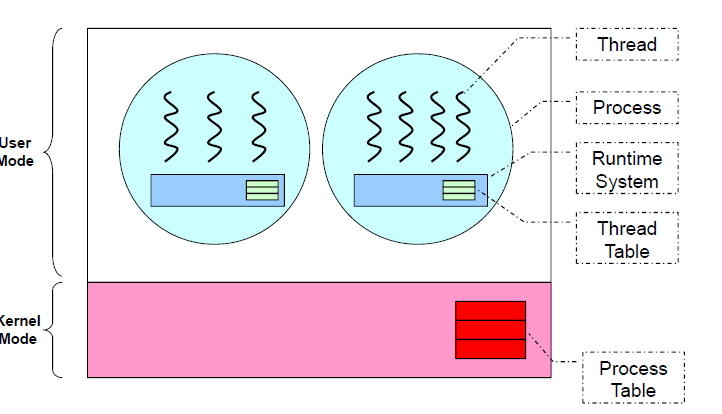
\includegraphics[width=0.4\textwidth]{4_1.png}
\end{figure}
The advantages of user thread model are
\begin{itemize}
  \item Can have multithreaded process on \textit{any} OS
  \item Thread operations are just library calls
  \item Generally more configurable and flexible, e.g. the scheduling algorithm can be customized.
\end{itemize}
However, the disadvantages are
\begin{itemize}
  \item OS is not aware of threads, therefore the scheduling of threads across processes is performed at process level. Therefore, one thread blocked will cause the process to be blocked, and therefore all other process will be blocked
  \item It cannot exploit multiple CPUs.
\end{itemize}
\end{definition}
\begin{definition}[Kernel Thread]
\hfill\\\normalfont Thread is implemented in the OS, and thread operation is handled as system calls.\\
This makes thread-level scheduling possible, and kernel may make use of threads for its own execution.
\begin{figure}[h]
\centering
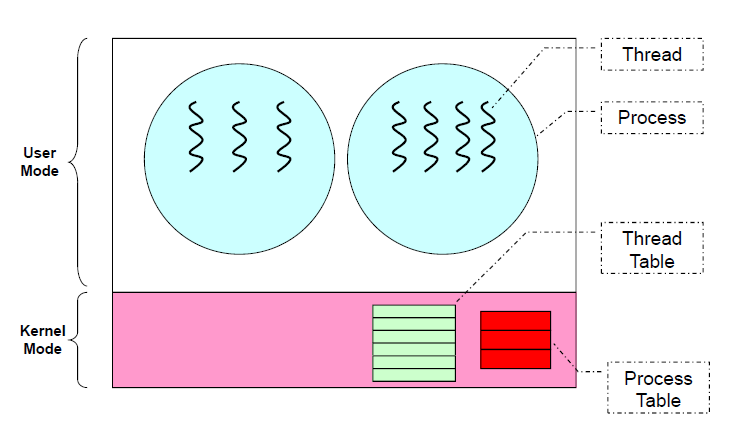
\includegraphics[width=0.4\textwidth]{4_2.png}
\end{figure}
The advantages of kernel thread model are
\begin{itemize}
  \item Kernel can schedule on thread levels, therefore more than 1 thread in the same process can run simultaneously on multiple CPUs.
\end{itemize}
However, the disadvantages are
\begin{itemize}
  \item Thread operations is now a system call, which is slower, and more resource intensive
  \item If implemented with many features, then it will be expensive and an overkill for simple program
  \item If implemented with few features, it is not flexible enough for some programs
\end{itemize}
\end{definition}
To take advantage of both models, in actual system, we use a hybrid thread model, where
\begin{itemize}
  \item there are both kernel and user threads
  \begin{itemize}
    \item OS schedule on kernel threads only
    \item User threads are binded to kernel threads
  \end{itemize}
\end{itemize}
\begin{figure}[h]
\centering
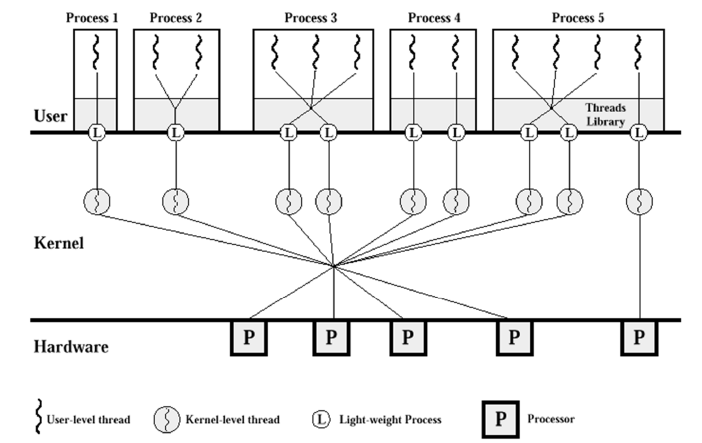
\includegraphics[width=0.4\textwidth]{4_3.png}
\end{figure}
This offers great flexibility, as we can limit the concurrency of any process/user.\\
Threads on a modern processor starts of a software mechanism and now become hardware native.
\subsection{POSIX Threads}
The thread in POSIX system can be used by including \texttt{\#include <pthread.h>}. The useful datatypes are
\begin{itemize}
  \item \texttt{pthread\_t}: data type to represent a thread id
  \item \texttt{pthread\_attr}: data type to represent attributes of a thread
\end{itemize}
Creation of a thread is done through
\texttt{pthread\_create(pthread\_t* tidCreated, const pthread\_attr\_t* threadAttributes, void* (*startRoutine) (void*), void* argForStartRoutine)}\\
This call returns $0$ for success and non-zero for errors.\\
Termination of a thread is done through
\texttt{int pthread\_exit(void* exitValue)}\\
Here, \texttt{exitValue} is the value to be returned to whoever synchronize with this thread. If it is not called, a pthread will terminate automatically at the end of startRountine, with no exit value returned.\\

Thread synchronizatin is done via
\texttt{int pthread\_join(pthread\_t threadID, void \*\*status)}\\
which waits for the termination of another pthread. It returns $0$ for success and nonzero for errors.

\section{Inter-Process Communication(IPC)}
Since it is hard for cooperating process to share information, we need IPC mechanisms. There are two common IPC mechanisms, namely \textbf{shared memory} and \textbf{message passing}. There are two \textit{Unix-specific} IPC mechanisms, namely \textbf{pipe} and \textbf{signal}.
\subsection{Shared Memory}
Communication via \textbf{shared memory} is done via the following steps:
\begin{itemize}
  \item Process $P_1$ \underline{creates} a shared memory region $M$.
  \item Process $P_2$ \underline{attaches} memory region $M$ to its own memory space.
  \item $P_1$ and $P_2$ can now communicate using this memory region $M$.
\end{itemize}
The same model is also applicable to multiple processes haring same memory region.\\
The advantages of shared memory scheme are
\begin{itemize}
  \item \textbf{Efficient}, since only initial steps of creation and attachment involves PS
  \item \textbf{Easy to use}, since shared memory region behaves the same as normal memory space, so information of any size or type can be written easily.
\end{itemize}
The disadvantages are
\begin{itemize}
  \item \textbf{Synchronization}: Since it is shared resource, we need to have a proper way for synchronized access
  \item \textbf{Harder Implementation}.
\end{itemize}
For POSIX Shared Memory sheme, after the steps outlined above,
\begin{itemize}
  \item Detach $M$ from memory space after use
  \item Destory $M$. For this destory operation, only one process needs to do this, and it can only be done if $M$ is not attached to any process
\end{itemize}
\subsection{Message Passing}
Communication via \textbf{Message Passing} is done via the following steps:
\begin{itemize}
  \item Process $P_1$ prepares a message $M$ and send it to process $P_2$.
  \item Proecss $P_2$ receives the message $M$
  \item Message sending and receiving are usually provided as system calls
\end{itemize}
For this model, we need to concern about
\begin{itemize}
  \item \textbf{Naming}: how to identify the other party in the communication
  \item \textbf{Synchronization}: the behaviour of sending/receiving operations
\end{itemize}
Essentially, since OS is involved in message passing(sending and receiving), the message \textit{have to} be stored in kernel memory space.\\
There are two naming shemes:
\begin{definition}[Direct Communication]
\hfill\\\normalfont Sender/Receiver of the message explicitly name the other party. For example, \texttt{Send(P2, Msg); Receive(P1, Msg)}.\\
The characteristics of this scheme are
\begin{itemize}
  \item We need one link per pair of communicating processes
  \item We need to know the identity of the other party
\end{itemize}
\end{definition}
\begin{definition}[Indirect Communication]
\hfill\\\normalfont Message are sent to/received from message storage, usually known as \textbf{mailbox} or \textbf{port}. All messages are sent or retrieved from mailboxes.\\
The characteristics of this scheme is that one mailbox can be shared among a number of processes.
\end{definition}
There are also two synchronization behaviours:
\begin{definition}[Blocking Primitives(Synchronous)]
\hfill\\\normalfont 
\begin{itemize}
  \item \texttt{Send()} will cause sender to be blocked until the message is received.
  \item \texttt{Receive()} will cause receiver to be blocked until a message arrives.
\end{itemize}
\end{definition} 
\begin{definition}[Non-Blocking Primitives(Asynchronous)]
\hfill\\\normalfont 
\begin{itemize}
  \item \texttt{Send()} will have sender resume operation immediately.
  \item On \texttt{Receive()}, receiver either receive the message if available, or some indication that message is not ready yet.
\end{itemize}
\end{definition} 
The advantages of message passing is that
\begin{itemize}
  \item \textbf{Portable}: can easily be implemented on different processing environment
  \item \textbf{Easier Synchronization}: especially synchronous primitive is used, sender and receiver are implicitly synchronized.
\end{itemize}
The disadvantages are 
\begin{itemize}
  \item \textbf{Inefficient}, as it requires OS intervention
  \item \textbf{Harder to use}, as message are usually limited in size and/or format
\end{itemize}
\subsection{UNIX Pipes}
In Unix, a proces has 3 default comminucation channels:
\begin{itemize}
  \item stdin
  \item stderr
  \item stdout
\end{itemize}
Unix shell provides the ``$\mid$'' symbol to link the input/output channels of one process to another, and this is known as \textbf{piping}.\\
Essentially, a pipe can be shared between two processes, which makes the two processes to form a Producer-Consumer relationship.\\
The pipe behaves like an anonymous file, and access of this pipe is FIFO, i.e. access of data must be in order.\\

In implementation, pipe functions are implemented as \textbf{circular bounded byte buffer} with implicit synchronization:
\begin{itemize}
\item Writer will wait when buffer is full
\item Reader will wait when buffer is empty
\end{itemize} 
\textbf{Remark}: In variants of pipe, we can have multiple readers and writers. Also, the pipe can be either \textbf{half-duplex} or \textbf{full-duplex}.\\

The \texttt{C} system call is \texttt{int pipe(int fd[])}, where \texttt{fd[0]} is the reading end and \texttt{fd[1]} the writing end.\\

If we wan tto change the standard communication channels, we can use system calls named \texttt{dup()} and \texttt{dup2()}.
\subsection{Unix Signal}
Unix Signal is a form of inter-process communication, which serves as an asynchronous notification regarding an event sent to a process or a thread.\\
The recipient of the signal must handle the signal, by
\begin{itemize}
  \item A default set of handlers, or
  \item User supplied handler(only applicable to some signals)
\end{itemize}
The common signals in UNIX include kill, stop, continue, memory error, arithmetic error etc.

\section{Synchronization}
The lack of synchronization will cause problem with \textbf{shared, modifiable resources} when concurrent processes access it in a interleaved fashion. This is known as \textbf{race condition}.\\
To resolve this, we need to implement a \textbf{critical section} where only one process can enter at any time. Correct Critical Section requires the following properties to be satisfied:
\begin{enumerate}
  \item \textbf{Mutual Exclusion}: If process $P_1$ is executing in critical section, all other processes are prevented from entering the critical section
  \item \textbf{Progress}: If no progress is in a critical section, one of the waiting processes should be granted access.
  \item \textbf{Bounded Wait}: After process $P_1$ request to enter critical section, there exists an upper bound of number of times other process can enter the critical section before $P_1$.
  \item \textbf{Independence}: Process \textit{not} executing in critical section should never block other process. 
\end{enumerate}
In case of incorrect synchronization, there will be problems like
\begin{enumerate}
  \item Deadlock, where all processes are blocked
  \item Livelock, where processes keep changing state to avoid deadlock and make no other progress
  \item Starvation, where some processes are blocked forever
\end{enumerate}
\subsection{Assembly Level Implementation}
We require an \textbf{atomic} instruction, named \texttt{TestAndSet}:
\[
\texttt{TestAndSet Register, MemoryLocation}
\]
The behaviour of the \texttt{TestAndSet} is to 
\begin{enumerate}
  \item Load the current content at \texttt{MemoryLocation} into \texttt{Register}
  \item Stores a $1$ into \texttt{MemoryLocation}
  \item Returns the Register's value to the user
\end{enumerate}
Therefore, \texttt{TestAndSet} will return $1$ if and only if the resource is used by another process.\\
With this observation, we can code \texttt{EnterCS} and \texttt{ExitCS} as follow:
\begin{verbatim}
void EnterCS(int* lock){
    while(TestAndSet(lock)==1);
}
void ExitCS(int* lock){
    *lock = 0;
}
\end{verbatim}
The implementation satisfies all four requirement of critical section, but the drawback is also evident: it employs a \textbf{busy waiting} scheme when waiting to enter CS, which is a wasteful use of processing power. We hope that such wait can essentially be turned into a blocked state of the process.
\subsection{High Level Language Implementation}
\begin{theorem}[Peterson's Algorithm]
\hfill\\\normalfont Suppose there are two processes $P_0$ and $P_1$. We will use 
\begin{enumerate}
  \item \texttt{Turn}, a variable that is set to indicate the turn belongs to the other process before checking for whether it is permitted to enter critical section
  \item \texttt{Want} array of 2 elements. This \texttt{Want} array allows process to indicate the intention of entering the critical section.
\end{enumerate}
Suppose process $0$ wants to enter critical section, it will set \texttt{Want[0]=1} and \texttt{Turn=1}, and check whether \texttt{Want[1]\&\&Turn==1} is true, which means that opponent wants and has the turn to use the critical section. If it is true, it will use a while loop to block $P_0$'s entrance.\\
After it successfully finishes critical section, \texttt{Want[0]=0}.
\end{theorem}
The assumption here is \textbf{writing to turn} is \textbf{atomic}.\\
The drawback of this algorithm is 
\begin{itemize}
  \item Buzy Waiting
  \item Low level
  \item Not general, as we may require more than mutual exclusion for synchronization
\end{itemize}
\subsection{High Level Synchronization Mechanism}
\begin{definition}[Semaphore]
\hfill\\\normalfont A semaphore is a generalized synchronization mechanism, which provides 
\begin{itemize}
  \item a way to block a number of processes, known as \textbf{sleeping process}, and 
  \item a way to unblock/wake up one, or more sleeping process
\end{itemize}
Semaphore will contain a integer valued number $S$. This $S$ can be initialized to any non-negative values initially.\\
Semaphore supports two \textbf{atomic} semaphore operations: \texttt{Wait(S)} and \texttt{Signal(S)}.
\begin{verbatim}
Wait(S)
    if(S<=0) blocks
    decrement S
Signal(S)
    increment S
    wake up one sleeping process if any
\end{verbatim}
The invariant of semaphore is
\[
S_\text{current} = S_\text{initial} + \#\text{signal}(S) - \#\text{wait}(S)
\]
where $\#\text{signal}(S)$ is number of signals operations executed, and $\#\text{wait}(S)$ is the number of wait operation \textbf{completed}.\\
With this invariance, we have $S_\text{current}+N_\text{CS}=1$ for binary semaphore. This ensures there is no deadlock.
\end{definition}
\subsection{Classical Synchronization Problems}
\subsubsection{Producer Consumer}
Suppose there is a shared bounded buffer of size $K$, where producer can produce item into the buffer if buffer is not full, and consumers can remove item from the buffer if buffer is not empty. There are multiple consumers and multiple producers.
\begin{figure}[h]
\centering
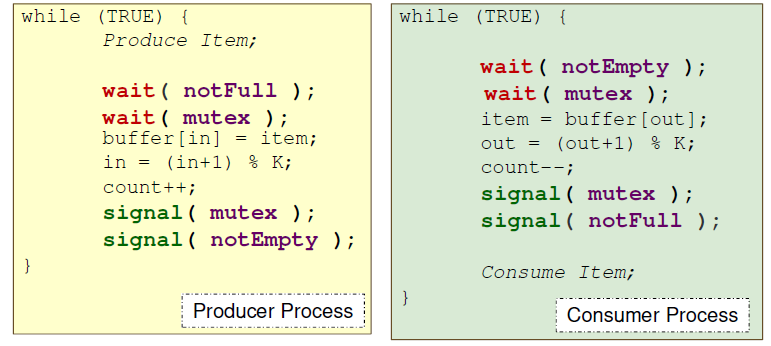
\includegraphics[width=0.4\textwidth]{5_1.png}
\end{figure}
is a blocking solution, if we initialize count, in , out to be $0$ and mutex has $S=1$, notFull has $S=K$ and notEmpty has $S=0$.
\subsubsection{Reader Writer}
Suppose there is a data structure $D$ where reader can retrieves information from $D$ and writer can modify information from $D$. Here we grant writer \textbf{exclusive access} to $D$, whereas multiple readers can access at the same time.
\begin{figure}[h]
\centering
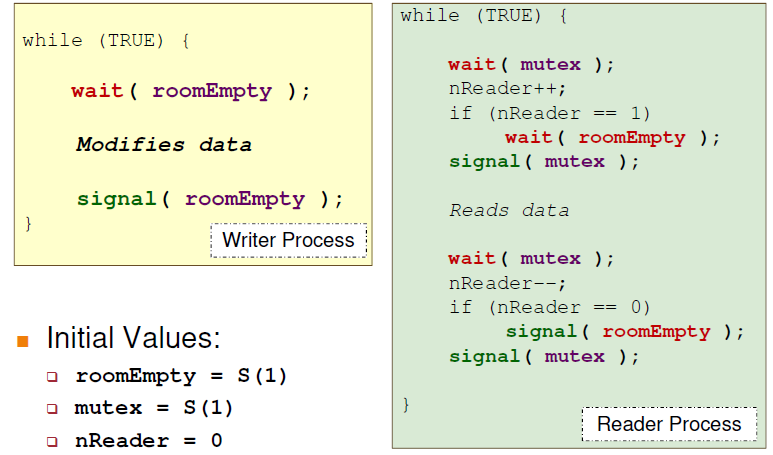
\includegraphics[width=0.4\textwidth]{5_2.png}
\end{figure}
is a solution that favours reader.
\subsubsection{Dining Philosophers}
There are 5 philosophers seating around the table, either thinking, hungry or eating. There is one chopstick to the left and another to the right of each philosopher, in total 5. We aim to let some of the philosopher to dine by successfully taking up 2 chopsticks that is on its left and right.\\
The code is detailed in the lecture notes.\\
An alternative is to use limited eater, where will use a semaphore with $S=4$ to limit number of seats to 4. and we use a semaphore on each chopsticks.

\section{Memory Abstraction}
Memory is an array of bytes, with a unique index for each byte, known as physical address. For process, there are 4 regions: text, data, heap and stack. Out of these 4, how text and data are layed outis decided by compiler in executable.\\
There are two types of data in a process:
\begin{itemize}
  \item \textbf{Transient} data, which is valid only for a limited duration, e.g. function parameter, local variable
  \item \textbf{Persistent} data, which is valid for duration of program unless explicitly removed, e.g. global variable, constant variable, dynamically allocated memory
\end{itemize}
Note: both types of data section can grow/shrink during execution.
\subsection{Memory Abstraction}
Without memory abstraction, memory access is straightforward, as address is fixed during compilation time, and such address is the physical address. However, different process may face conflict and it is also hard to protect memory space. \\
One simple abstraction is the usage of base and limit registers.
\begin{definition}[Base and Limit Registers]
\hfill\\\normalfont Use a special register as base of all memory references, which is known as \textbf{base register}. During compilation time, all memory references are compiled as \textit{offset} from this register. At loading time the base register is initialized as the starting address of the process memory space.\\
Use another special register to indicate the range of the memory space of the current process, which is known as \textbf{limit register}. All memory access is checked against the limit to protect memory space integrity.
\end{definition}
The problem with this approach is that to access any address, we need to do more computations:
\begin{itemize}
\item $\texttt{Actual}=\texttt{Base}+\texttt{Adr}$ to get actual address.
\item Check $\texttt{Actual}<\texttt{Limit}$ for validity.
\end{itemize}
The idea evolves to be the idea of \textbf{logical address}, which has a bijection to physical address. Building on this abstraction, each process will now have a self-contained, independent logical memory space.
\subsection{Contiguous Memory Management}
In this subsection, we assume
\begin{enumerate}
  \item Each process occupies a \textbf{contiguous memory region}.
  \item The \textbf{physical memory is large enough} to contain one or more processes with complete memory space.
\end{enumerate}
Here, to support multitasking, we allow multiple process to be in the physical memory at the same time for efficient switching. When physical memory is full, we free up memory by
\begin{itemize}
\item  removing terminated process, or 
\item swapping blocked process to secondary storage.
\end{itemize}
\begin{definition}[Memory Partition]
\hfill\\\normalfont Memory Partition is the contiguous memory region allocated to a single process.
\end{definition}
We can make these partitions in two ways, either \textbf{fixed-sized partition} or \textbf{variable-sized partition}.\\
\begin{definition}[Fixed Sized Partition]
\hfill\\\normalfont For fixed sized partition, physical memory is split into fixed number of equally sized partition and a process will occupy one of them.\\
It has the advantage of easy management and fast allocation. However, partition size need to be large enough to contain the largest of the processes.\\
Therefore, smaller process will waste memory space, known as \textbf{internal fragmentation}.
\end{definition}
\begin{definition}[Dynamic Partitioning]
\hfill\\\normalfont For variable-sized partition, partition is created based on actual size of process. OS keep track of the state of occupied and free memory regions and perform splitting and merging when necessary.\\
It is flexible and avoid internal fragmentation, but OS needs to maintain more information, and it takes more time to locate appropriate region. Also, \textbf{external fragmentation} occurs, which creates a large number of holes.
\end{definition}
The allocation algorithm for dynamic partitioning can be
\begin{itemize}
  \item First fit: take the first large-enough hole
  \item Best fit: find the smallest hole that is large-enough
  \item Worst fit: find the largest hole
  \end{itemize}
After finding the hole, split.\\
When occupied partition is freed, algorithm will merge it with adjacenet hole if available.\\
Suppose the holes are fragmented, \textbf{compaction} can be used to move the occupied partition around to create consolidate holes.\\
The OS usually stores the memory information into a linked list of 3-tuple: (\texttt{Status}, \texttt{Start Address}, \texttt{Length}).
\begin{theorem}[Buddy System]
\hfill\\\normalfont Buddy memory allocation provides efficient
\begin{itemize}
  \item Partition Splitting
  \item Locating good match of free partition
  \item Partition de-allocation and coalescing
\end{itemize}
Suppose memory is of $2^K$ byte, we keep an array of \texttt{A[0..K]}. Each array element \texttt{A[j]} is a linked list which keep tracks of \textbf{free} blocks of size $2^j$. Each free block is indicated by the starting address.\\
To allocate a block of size $N$, 
\begin{enumerate}
  \item Find smallest $S$ such that $2^S\geq N$.
  \item Access \texttt{A[S]} for a free block.
  \begin{enumerate}
    \item If free block exists, remove block from \texttt{A[S]} and allocate
    \item Else, find the smallest \texttt{R} from \texttt{S+1} to \texttt{K}, such that \texttt{A[R]} has a free block $B$. Repeatedly split $B$ until there are free blocks in \texttt{A[S]} and allocate.
  \end{enumerate}
\end{enumerate}
To deallocate a block $B$, 
\begin{enumerate}
  \item Check in \texttt{A[S]}, for the buddy of $B$, say $C$. If it exists, remove $B$ and $C$, and merge to $B'$, and try deallocate $B'$.
  \item Else, insert $B$ in \texttt{A[S]}.
\end{enumerate}
\end{theorem}
Note, two blocks are buddy of size $2^S$, if the $S$ bit of $B$ and $C$ is a complement and leading bits up to $S$th bit of $B$ and $C$ are the same.

\section{Disjoint Memory Schemes}
In this section, process memory space can now be in \textbf{disjoint physical memory locations}. This can be done via paging or segmentation.
\subsection{Paging}
The \textbf{physical memory} is split into regoins of fixed size, known as \textbf{physical frame}. The \textbf{logical memory}, which has same size as physical, is also split into regions of \textit{same size}, known as \textbf{logical page}.\\
At execution time, pages of a process are loaded into \textit{any available} memory frame. The process will still occupy a contiguous logical memory space.\\
Under paging scheme, we will keep a mapping of logical page to corresponding physical frame using \textbf{page table}. Essentiallly, the logical memory of a process always start with page $0$, so the page table $\texttt{Table}$ can be an $0$-indexed array.\\
Suppose the physical frame size, which is also page size, equals $S$, then the physical address of $k$th byte of $i$th page equals $\texttt{Table}[i]\times S+k$.\\
In practice, we 
\begin{itemize}
  \item Keep frame size and page size as power-of-2
  \item Also, physical frame size equals logical page size
\end{itemize}
Suppose we have $2^n$ bytes in a page, then the logical address can be represented by $\underbrace{p}_{(m-n)}\underbrace{d}_{n}$. The corresponding physical address is $\underbrace{f}_{(m-n)}\underbrace{d}_{n}$, where $f=\texttt{Table}[p]$.\\

Paging removes \textbf{external fragmentation}, but there exists, still, \textbf{internal fragmentation}.\\

To implement efficient paging scheme, we need \textbf{translation look-aside buffer}(TLB). TLB is a cache of a \textit{few} page table entries.\\
TLB works as below:
\begin{itemize}
  \item Page number is used to search TLB associatively (in parallel)
  \item If TLB hit, then frame number is retrieved for translation
  \item If TLB miss, memory access is done to access the full page table, update TLB and do translation
\end{itemize}
When a context swtich occurs, TLB entries are flushed. When process is switched back, TLB miss will occur to fill TLB. It is still possible to place some entries initially, like the code pages, to reduce TLB misses.\\

Paging scheme can provide protection of memory using access-right bits and valid bit.\\
Access Right bit is attached to each page table entries to indicate whether it is writable, readable or executable. Memory access is checked against the access right bits.\\
Valid bit is attached to each page table entry to indicate whether the page is valid for process to access. This bit is set by OS and out-of-range will be caught.\\
The page table allows several processes to share the same physical frame, by putting the same physical frame number in page table entries. Therefore, it can be used to 
\begin{itemize}
  \item Share code page
  \item Implement copy-on-write
\end{itemize}
\subsection{Segmentation Scheme}
It is hard to place different regions(data, text, stack, heap) in contiguous memory space, physical or logical, and allow growing/shrinking freely. Therefore, we use \textbf{segmentation scheme}, which separate regions into multiple memory segments. Logical memory space is then a collection of segments.\\
Each memory segment will have a name, and have a limit to indicate the range. The memory reference is now specified as \texttt{segment name + offset}.\\
Each process will keep track of a \textbf{segment table}, whjich is a mapping between different segments, identified by \texttt{segID} to a pair: \texttt{<Base, Limit>}. Suppose the logical address is \texttt{SegID} with offset $k$, then the physical address is \texttt{Table[SegID]+k}, if $k$ is less than limit. \\
Since we need to check limit and also do addition for offset, we do not hardware to support these operations.\\
Segmentation scheme is good since each segment can grow/shrink independently and can be protected/shared independently.\\
However, segmentatino requires variable-size contiguous memory regions, which can cause external fragmentation.\\
\subsection{Segmentation with Paging}
The idea is to page each segment.
\begin{figure}[h]
\centering
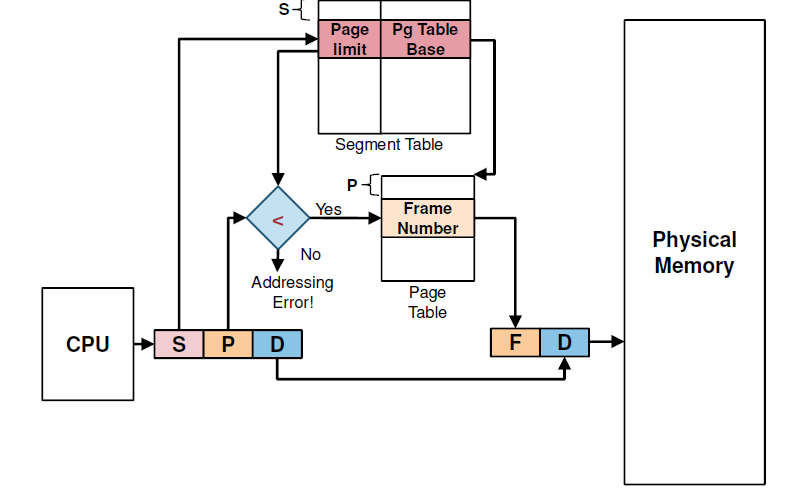
\includegraphics[width = 0.4\textwidth]{8_1.png}
\end{figure}

\section{Virtual Memory Management}
In virtual memory management, we allow logical memory space of a process tobe larger than physical memory. The logical address space can either reside in physical memory or in \textit{secondary} storage.\\
We extend the paging scheme:
\begin{itemize}
  \item Logical memory space is split into fixed size page
  \item Some pages may be in physical memory
  \item Others in secondary storage
\end{itemize}
We use a \textbf{page table} to translate virtual address to physical address. In the page table, we add an additional field to distinguish between a \textbf{memory resident} and non-memory resident.\\
If CPU finds out a certain page is \textit{not} memory resident, it will trigger a \textbf{page fault}, which will be handled by OS, to bring the non-memory resident page into the physical memory. After this step, CPU will retry the instruction. 
\begin{figure}[h]
\centering
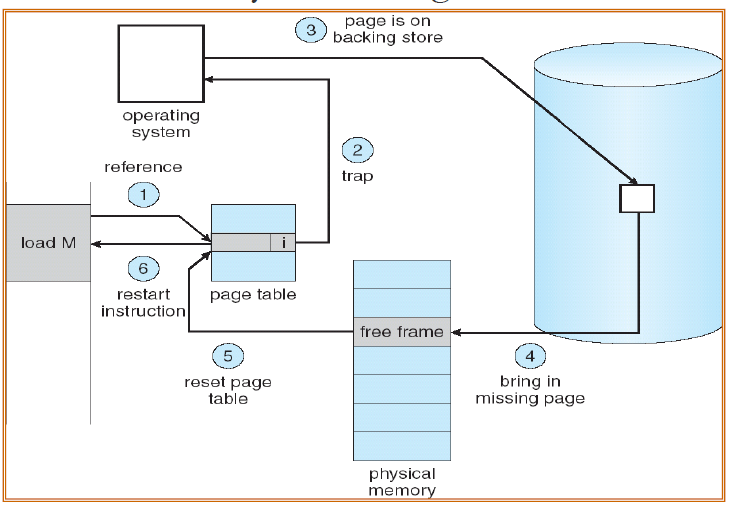
\includegraphics[width=0.4\textwidth]{9_1.png}
\end{figure}
It is usually unlikely that \textbf{thrashing}, the occurrence of page fault, will happen, because of \textbf{locality principle}, which includes temporal and spatial locality.\\
\begin{itemize}
  \item Temporal Locality: after a page is loaded to physical memory, it is likely to be accessed in near future, so that cost of loading page is amortized.
  \item Spatial Locality: a page contains contiguous locations that is likely to be accessed in near future, so later access to nearby locations will not cause page fault.
\end{itemize}
Virtual memory completely separate logical memory address from physical memory, as amount of physical memory no longer restrict the size of logical memory address.\\
It is a more efficient use of physical memory, as page currently not needed can be on secondary storage.\\
It allows, also, more proecsses to reside in memory, so that more processes can be chosen to run by CPU, increasing CPU utilization.
\subsection{Page Table Structure}
In case of huge memory space, page table via \textbf{direct paging} will also be huge, and remain fragmented in different pages. Therefore, we need a neater design of page table.\\
\begin{definition}[2-Level Paging]
\hfill\\\normalfont We split the full page table into smaller page tables, each with a \textbf{page table number}. If the original page table has $2^P$ entries, with $2^M$ smaller page tables, $M$ bits is needed to unique identify one page table; each smaller page table contains $2^{P-M}$ entries.\\
Each smaller page table should ideally be of the same size as the page size, to avoid page fault.
To keep track of these smaller page tables, a single \textbf{page directory} is needed, which contains the $2^M$ indices to locate each of the smaller page table.
\begin{figure}[h]
\centering
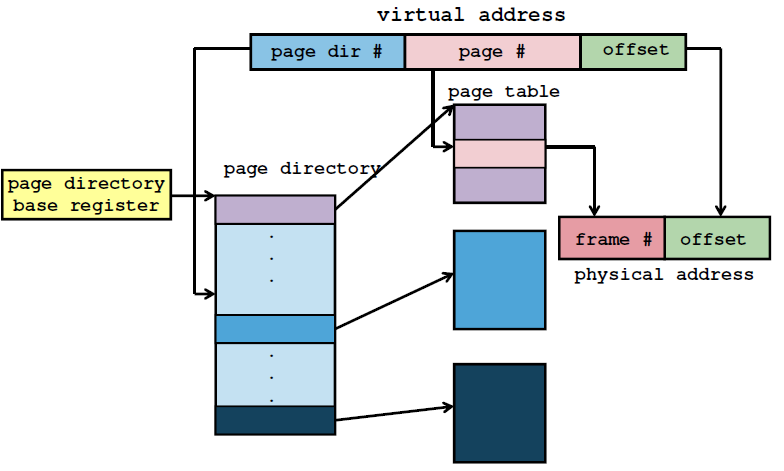
\includegraphics[width=0.4\textwidth]{9_2.png}
\end{figure}
\end{definition}
It allows empty entries in the page directory, which means the corresponding smaller page table need not be allocated. This saves memory space.
\begin{definition}[Inverted Page Table]
\hfill\\\normalfont Normal page table is per-process information. Also, mapping from physical frame to logical memory is inaccessible.\\
\textbf{Inverted Page Table} keeps a \textbf{single} mapping of physical frame to $\langle \text{pid}, \text{page number}\rangle$. Here, the page number is specific to the pid.\\
The offset of the inverted page table entry will be the frame number of physical frames.\\
To make query faster, one should hash the inverted page table.
\begin{figure}[h]
\centering
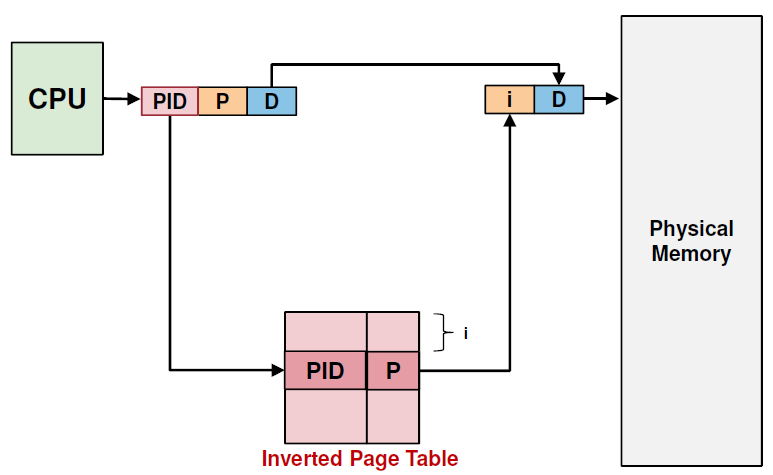
\includegraphics[width=0.4\textwidth]{9_3.png}
\end{figure}
\end{definition}
\subsection{Page Replacement Algorithm}
In the case of page fault, we need to evict(free) a memory page, by writing back the old page to the memory if the page id modified, therefore \textbf{dirty}.\\
To decide which page to evict, we need to look at a suitable replacement algorithm. A good replacement algorithm should \textbf{reduce the total number of page faults}.
\begin{definition}[Optimum]
\hfill\\\normalfont Optimum page replacement algorithm replace the page that \textbf{will not be used again for the longest period of time}.
\begin{itemize}
\item If the page is in memory, only update \textbf{next use time}.
\item Else, 
\begin{itemize}
  \item If memory is not full, load it and update \textbf{next use time}.
  \item Else, choose the existing page with largest next use time to evict, and load the new page.
\end{itemize}
\end{itemize}
This guarantees minimum number of page faults.\\
However, it is not realizable, due to requirement of future knowledge of memory access.
\end{definition}
\begin{definition}[FIFO Page Replacement]
\hfill\\\normalfont Memory pages are evicted based on their loading time. One evicts the oldest memory page. Therefore, 
\item If the page is in memory, use.
\item Else, 
\begin{itemize}
  \item If memory is not full, load it and update \textbf{loaded-at time}.
  \item Else, choose the existing page with smallest loaded-at time to evict, and load the new page.
\end{itemize}
The problem with FIFO algorithm is Belay's Anomaly, where the number of page fault can increase if the number of physical frame increases. The reason is FIFO does not exploit temporal locality. 
\end{definition}
\begin{definition}[Least Recently Used(LRU)]
\hfill\\\normalfont In LRU, we replace the page that has not been used in the longest time. It avoids Belady's Anomaly.
\item If the page is in memory, only update \textbf{last use time}.
\item Else, 
\begin{itemize}
  \item If memory is not full, load it and update \textbf{last use time}.
  \item Else, choose the existing page with smallest last use time to evict, and load the new page.
\end{itemize}
However, implementing LRU is not easy, because the last use time can overflow, and also the searching of smallest last use time page requires a complete search.
\end{definition}
\begin{definition}[Second-Change Page Replacement]
\hfill\\\normalfont It used a modified FIFO to give a second chanmge to pages that are accessed. We need the page table entry to maintain a reference bit:
\begin{itemize}
  \item $1=\text{Accessed}$
  \item $0=\text{Not Accessed}$.
\end{itemize}
\begin{itemize}
\item Initialize the next victim pointer to the first frame when it is loaded.
\item If the page is in memory, set reference bit to $1$.
\item Else, 
\begin{itemize}
  \item If memory is not full, load it and set reference bit to $0$.
  \item Else, we look at the next victim pointer.
  \begin{itemize}
    \item If next victim pointer points to a page with reference bit $0$, replace that page.
    \item Else, advance victim pointer and check again.
    \item If all pages have reference bit $1$, change the original victim to the new page.
  \end{itemize}
\end{itemize}
\end{itemize}
\end{definition}
\subsection{Frame Allocation}
To allocate $N$ physical memory frames among $M$ processes, some simple appoaches can be
\begin{itemize}
  \item Equal distribution
  \item Proportional allocation to the size of process.
\end{itemize}
During page replacement, if victim page is selected among \textbf{page of the same process} that causes page fault, it is known as \textbf{local replacement}. Otherwise, it is known as \textbf{global replacement}.\\
Local Replacement has advantage of stable performance between multiple runs, since number of pages allocated remains constant.\\However, it has disadvantage of potentially hindering the progress of a process if page is not allocated enough.\\
Global Replacement has the advantage of allowing self-adjustment between processes, so that process that needs more frame can get from others.\\ However, badly behaving process can affect others.\\
If global replacement is used, 
\begin{itemize}
  \item Thrashing steals page from other process, which can cause cascading thrashing
\end{itemize}
If local replacement is used,
\begin{itemize}
  \item Although thrashing is localized, single process doing thrashing can hog the I/O and degrades performance of other processes.
\end{itemize}
\begin{definition}[Working Set Model]
\hfill\\\normalfont We define the working set Window $\delta$ as a interval of time. We denote $W(t,\delta)$ to be the active pages in interval at time $t$. We allocate enough frames for pages in $W(t,\delta)$ to reduce possibility of page fault.\\
The accurancy of working set model is directly affected by the $\delta$ chosen.
\end{definition}

\section{File Management Introduction}
We want to introduce a file system on top of external storage to store \textbf{persistent} information, in contrast to physical memory storing \textbf{volatile} information.\\
File system sdhould provide
\begin{itemize}
  \item Abstraction on top of physical media
  \item A high level resource management scheme
  \item Protection between processes and users
  \item Sharing between processes and users
\end{itemize}
The requirement of file system needs to be
\begin{itemize}
  \item \textbf{self-contained}, where information stored on a media is enough to describe the entire organization; should be able to ``plug and play'' on another system
  \item \textbf{Persistent}: data should persist beyond the lifetime of OS and processes
  \item \textbf{Efficient}: it should provide good management of free and used space, and there should be minimum overhead for bookkeeping information
\end{itemize}
\subsection{File System Abstractions}
File System consists of a collection of \textbf{files} and \textbf{directory} structures, where
\begin{itemize}
  \item \textbf{File}: an abstract storage of data, and
  \item \textbf{Directory}: Organization of files
\end{itemize}
File systems provides an abstraction of accessing and using the files and directories.\\
File represents a logical unit of information created by process. It can be viewed as an abstract data type, in which there are
\begin{itemize}
  \item \textbf{Data}: Information structured in some ways
  \item \textbf{Metadata}: Additional Information associated with the file, also known as file attributes. Common metadata fields include 
  \begin{itemize}
    \item Name: a human readable reference to the file.\\Different file system will have different \textbf{naming rule}. Some system include file extension in file name like \texttt{Name.Extension} so as to use the extension to indicate \textbf{file type}.
    \item Identifier: A unique id for the file used internally by File System
    \item Type: indicate different type of files.\\
    There are 3 common file types:
    \begin{itemize}
      \item Regular files: contains user information. Inside regular files, there are two major types:
      \begin{itemize}
        \item ASCII files, which can be displayed as it is
        \item Binary files, which include executable, PDF files etc. It has a \textbf{predefined internal structure} that can be processed by specific programme.
      \end{itemize}
      We can use either \textbf{file extension}(windows) or \textbf{embedded information}(unix) to distinguish file types.
      \item Directories: system files for File System Structure
      \item Special files: character/block oriented
    \end{itemize}
    \item Size: current size of file
    \item Protection: Access permissions, can be classified as reading, writing and execution rights\\
    We can specify the type of access certain user or group of user can do on the file. The type of access include:
    \begin{itemize}
      \item Read: retrieve information from file
      \item Write: Write/rewrite the file
      \item Execute: Load file into memory and execute it
      \item Append: Add new information to the end of the file
      \item Delete: Remove file from File System
      \item List: Read metadata of the file
    \end{itemize}
    The most general scheme to specify these rights is to use a \textbf{access control list}, in the format of a list of user identity with their allowed access types. It is very customizabole but additional information needs to be associated with the file.\\
    Another way to protect the file is to use permission bits, covered in \texttt{CS2107.pdf}.
    \item Time, date and owner information: creation, last modification time, owner id etc
    \item Table of content: Infomration for the file system to determine how to access the file
  \end{itemize}
\end{itemize}
and various operations can be done on the file. \\
Operations that can be done on file metadata include:
\begin{itemize}
  \item Rename
  \item Change attributes, like file access permissions, dates, ownership etc
  \item Read attribute, like file creation time
\end{itemize}
File data can have three different ways for abstraction:
\begin{itemize}
  \item \textbf{Array of bytes}: there is no interpretatino of data, so the data are just raw bytes. Each byte has a unique offset from the file start.
  \item \textbf{Fixed length records}: array of records, which can grow/shrink. It can jump to any record easily since the offset of $n$th record is size of record$\times (n-1)$.
  \item \textbf{Variable length records}: which is flexible but harder to locate a record
\end{itemize}
There are also 3 kinds of access methods:
\begin{itemize}
  \item Sequential Access, which reads data in order, starting from beginning. Data cannot be skipped but can be rewound.
  \item Random Access, where data can be read in any order. This can be realized using
  \begin{itemize}
    \item \texttt{read(offset)}, which explicitly state the position to be accessed
    \item \texttt{seek(offset)}, which moves from old to a new location in the file. (used by windows and unix)
  \end{itemize}
  \item Direct Access: which is used for files that contains fixed-length records. It allow \textbf{random access to any record directly}. \\Basic random access method is a special case of direct access, where each record equals 1 byte.
\end{itemize}
There are a few operations that can be done on file data:
\begin{itemize}
  \item Create: create a new file with no data
  \item Open: perform before further operations, so as to prepare necessary information for file operations later
  \item Read: read data from file, usually starting from current position
  \item Write: write data to file, usually starting from current position
  \item Repositioning: which is seek.
  \item Truncate: removes data between specified position to the end of file
\end{itemize}
These operations are provided by OS via \textbf{system calls}, which provides protection, concurrent and efficient access, and also maintain necessary information. Especially, OS need to keep information for an \textbf{opened} file in a open-file table:
\begin{itemize}
  \item File Pointer: current location in file
  \item Disk Location: actual file location on disk
  \item Open Count: How many process has the file opened.
\end{itemize}
To keep track of these information, we need a system-wide open-file table and also some per-process open-file table. The system-wide table's entry corresponds to a unique file, whereas the per-process open-file table entry corresponds to a entry in a system-wide table.
\begin{figure}[h]
\centering
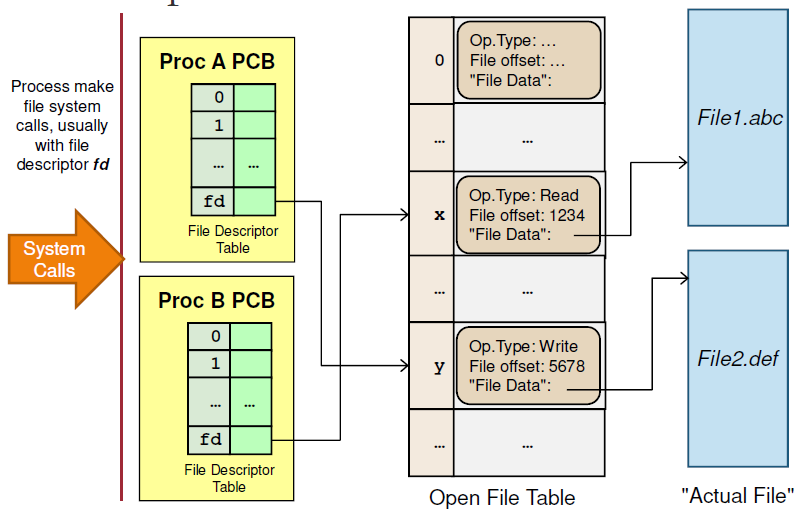
\includegraphics[width=0.4\textwidth]{10_1.png}
\end{figure}
\subsection{Directory}
Directory is used to
\begin{itemize}
  \item Provide a logical grouping of files
  \item Keep track of files
\end{itemize} 
We can structure the directory as 
\begin{itemize}
  \item Single-level
  \item Tree structure, which allows us to have an \textbf{absolute pathname}, and a \textbf{relative pathname} from the \textbf{current working directory}.
  \item DAG, by allowing files to be shared. This sharing can be done using
  \begin{itemize}
    \item Hard Link, which can only be used on files.\\
    A hard link of a file $F$ in directory $A$ to another directory $B$ makes $A$ and $B$ has separate pointers pointing to the actual file in disk. This has low overhead, since only pointers are added in directory, but deleting the file may cause problems. Hard link can be done using \texttt{ln}.
    \item Symbolic Link, which can be used on files and directory.\\ 
    In the same scenario above, now $B$ will create a \textbf{special link file} $G$ where $G$ contains the path name of $F$.When $G$ is accessed, it finds out where is $F$ and access $F$.\\
    This solves the problem of deletion, but has larger overhead. To achieve symbolic link, use \texttt{ln -s}.
  \end{itemize}
  \item General Graph\\
  This is not desirable, since we may encounter infinite loop in traversal and it is hard to determine when to remove a file or directory.
\end{itemize}

\section{File System Implementation}
General disk structure can be treated as a 1D array of \textbf{logical block}, where the logical block is the smallest accessible unit.\\Logical block is mapped into \textbf{disk sectors}, whose layout is \textbf{hardware dependent}.\\
The \textbf{Master Boot Record(MBR)} at sector $0$ with partition table, is followed by one or more partitions, where we 
put an independent file system in each partition.\\
A file system generally contains:
\begin{itemize}
  \item OS bootup infomration
  \item Partition details, e.g., total number of blocks and number and location of free disk blocks
  \item Directory structure
  \item File information
  \item Actual file data
\end{itemize}
\subsection{Implementing File}
File is a collection of logical blocks. Therefore, there could be internal fragmentation if the file size is not a integer multiple of logical blocks.\\
A good file implementation must
\begin{itemize}
  \item Keep track of logical blocks
  \item Allow efficient access
  \item Disk space is utilized effectively
\end{itemize}
\subsubsection{Contiguous Block Allocation}
In contiguous block allocation, we allocate consecutive disk blocks to a file.\\
It is simple to keep track of the file since we only need 
\begin{itemize}
  \item starting block number
  \item length
\end{itemize}
However, there will be external fragmentation, since we can leave holes as files get deleted.\\
Also, for this scheme, file size needs to e specified in advance.
\subsubsection{Linked List Allocation}
We keep a linked list of disk blocks, where each block stores:
\begin{itemize}
  \item The next disk block number
  \item Actual file data
\end{itemize}
The file information will store first and last disk block number.\\
Linked list implementation solves the external fragmentation, however,
\begin{itemize}
  \item Random access is very slow
  \item Part of the disk block is used for pointer
  \item Less reliable, since each pointer value can be a single point of failure
\end{itemize}
\subsubsection{Linked List v2.0}
Move all the block pointer into a single table, known as \textbf{File Allocation Table(FAT)}. The FAT is in \textit{memory} all the time.\\
This allows faster random access, since linkedlist traversal takes place in memory.\\
However, FAT keeps tracks of all disk block in a partition, so it can be huge when disk is large, and will consume valuable memory space.
\textbf{Remark}: For the Linked List Allocation, the last block is \textit{NULL}.
\subsubsection{Indexed Allocation}
In indexed allocation, each file has an \textbf{index block}, which is an array of disk block addresses, where \texttt{indexBlock[N]} is the $N$th block address.\\
The advantage is that we have lesser memory overhad, since only the indexed block of opened file needs to be in memory. This also allow fast direct access.\\
However, we have a limited maximum file size, since max number of blocks needs to be no larger than the number of index block entries. Also, there is a index block overhead.
\subsubsection{Indexed Allocation Variant}
We can use a linked scheme to keep a linkedlist of index block, where each index block contains the pointer to next index block.\\
We can also use multilevel index, where the higher level index block points to a number of lower level index blocks, and the leaf level index block point to actual disk blocks.
\subsection{Free Space Management}
We need to know the location of free space since we need these information for file allocation. Therefore, we should maintain a \textbf{free space list}, and support two functionalities:
\begin{itemize}
  \item Allocate, during free creation or enlargement
  \item Free, during file deletion and truncation
\end{itemize}
\subsubsection{Bitmap}
Each disk block can be represented by 1 bit in the bitmap, where $1$ means \textbf{free} and $0$ means \textbf{occupied}.\\
Bitset is good since it provides a good set of manipulations, however, we need to keep in memory the whole bitmap for efficiency reasons.
\subsubsection{LinkedList}
We can use a linked list of disk blocks, where each disk block contains a number of free disk block numbers and a pointer to the next free space disk block.
The linked list is stored in the free blocks themselves.
\subsection{Implementing Directory}
We need to 
\begin{itemize}
\item keep track of files and subdirectories in the directory, possibly with the file metadata
\item Map the file name to the file information
\end{itemize}
Given a full path name, we need to recursively search the directories along the path to arrive at the file information. \\
We can view subdirectory as a file entry with special type in the directory.
\subsubsection{Linear List Implementation}
Directory consists of a list, where each entry represents a file. The entry should contain
\begin{itemize}
  \item file name(minimum) and possibly other metadata
  \item file information or pointer to file information
\end{itemize}
Locating a file using list requires a linear search, which will be inefficient for large directories or deep tree traversal. To resolve this, we can use cache to remember the latest few searches.
\subsubsection{Hash Table}
Each directory contains a hash table of size $N$. When we locate a file by file name, we can use the hash.\\
It has fast lookup speed but hash table has limited size, and also the performance depends on good hash functions.
\\
For file information, it should consists of 
\begin{itemize}
  \item File name and otehr metadata
  \item Disk blocks information
\end{itemize}
We can 
\begin{itemize}
  \item Store everything in directory entry, or
  \item Store only file name and points to some data structure for other information
\end{itemize}
\subsection{File System in Action}
Previously, we concern about static information for a file system. However, at runtime, when user interacts with file, runtime information is needed, which should be maintained by OS in memory, e.g., system-wide and per-process open-file table, and buffer.
\subsubsection{FIle Creation}
We need directory structure to locate the parent directory. Search for filename to avoid duplicate. THe searching can be on cached directory structure.\\
Then we use free space list to find free disk blocks.\\
The we add an entry to parent directory, with relevant file information such as file name and disk block information.
\subsubsection{File Open}
\begin{enumerate}
  \item We first seafch system-wide table for existing entry. If found, create an entry in $P$'s table pointing to $E$ and return a pointer to this entry. If not, continue to next step.
  \item Use full pathname to lcoate file. If not found, terminate with error.
  \item When $F$ is located, its file infomration is loaded into a new entry $E$ in system-wide table
  \item Create an entry in $P$'s table to point to $E$, and return a pointer to this entry
\end{enumerate}
The returned pointer is used for further read/write operation.
\subsection{Disk I/O Scheduling}
The time taken to perform a read/write operation$=$ Seek time + Rotational Latency + Transfer Time.\\
The tiem taken to position the disk head over the proper track is known as \textbf{seek time}.\\
The time to wait for the desired sector to rotate under the read/write head is known as \textbf{rotational latency}.\\
The time taken to transfer the data is known as transfer time, which is $\frac{\text{Transfer size}}{\text{Transfer Rate}}$.\\
Usually, first two time are more significant than the third. Therefore it is worthwhile for OS to do scheduling. 
A few algorithms include
\begin{itemize}
  \item FCFS
  \item Shortest Seek First
  \item SCAN family, which can be bidirectional or unidirectional.
\end{itemize}

\section{File System Case Study}
\subsection{FAT File System}
\begin{figure}[h]
\centering
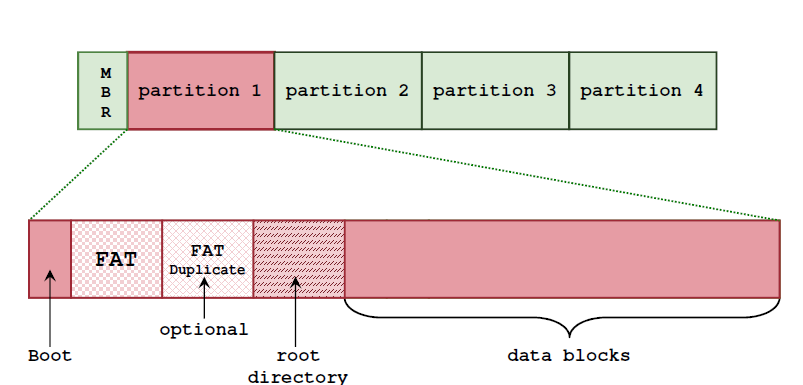
\includegraphics[width=0.4\textwidth]{12_1.png}
\end{figure}
Above, the FAT is called File Allocation Table.\\
File data are allocated to a number of data blocks, or data block cluster. The allocation info is kept as \textbf{linked list} and stored separately in the FAT.\\
In the FAT, there will be one entry per data-block/cluster. It stroes the block information such as whether theblock is free, next block, damaged etc.(see below)\\
OS will cache the FAT into the RAM to facilitate linked list traversal.\\
FAT entry contains either
\begin{itemize}
  \item FREE block
  \item Block Number of next book
  \item EOF code(i.e. NULL pointer)
  \item BAD block
\end{itemize}
Directory, on the other hand, is represented as a 
\begin{itemize}
  \item \textbf{special type of file}
  \item Root directory is stored in a \textit{special} location, whereas other directories are stored in data blocks
  \item Each file/subdirectory within the directory is represented as \textbf{directory entry}
\end{itemize}
Directory entry is a fixed-size 32-bytes per entry, which contains
\begin{itemize}
  \item Name, Extension
  \item Attributes
  \item Creation Date, Time
  \item First disk block, file size
\end{itemize}
\begin{figure}[h]
\centering
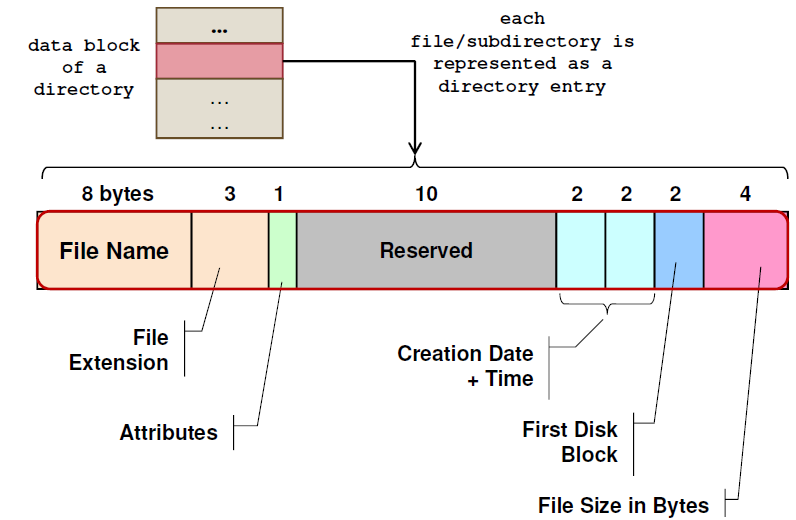
\includegraphics[width=0.4\textwidth]{12_2.png}
\end{figure}
\subsubsection{File Operations}
For \textbf{File Deletion}, we \textit{delete} teh directory entry by settting the first letter in the filename to the special value \texttt{0xE5}. We then free data blocks by setting FAT entries to FREE. However, actual data blocks remain intact.\\
However, we do not record the free spaces, so we must calculate it via traversal of FAT table.\\
Instead of pointing to the disk blocks, FAT indexes teh disk cluster. FAT32 allows $2^28$ clusters, subtracted by the special values for EOF etc. Cluster size will affect condition of internal fragmentation.\\
Virtual FAT adds in \textbf{long file name support}, that supports long filenames up to 255 characters. It use \textbf{multiple directory entries} for a file with long file name. It use a previously invalid file attribute so non-VFAT applications can ignore these additional entries. It also use teh first byte in the filename to indicate sequence.\\
The $8+3$ short version is kept for backward compatibility.
\subsection{Extended-2 File System}
Disk space is split into Blocks, and blocks are grouped into block groups. Each file/directory is described by a \textbf{single} special structure known as I-node(index node). I-node will contain file metadata and data block addresses.
\begin{figure}[h]
\centering
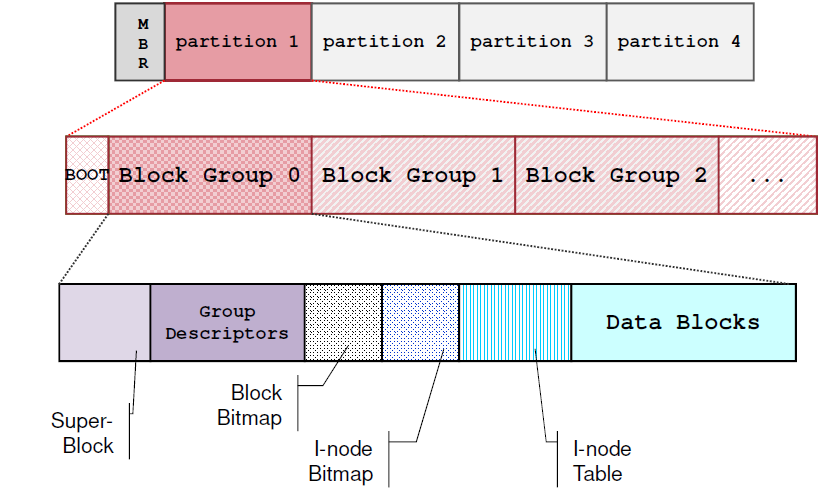
\includegraphics[width=0.4\textwidth]{12_4.png}
\end{figure}
\textbf{Superblock} descirbes the whole file system, for example total I-nodes number, I-node per group, total disk blocks, disk block sper group. This is duplicated in each block group for redundancy.\\
\textbf{Group descriptors} describe each block group, for example number of free disk blocks, free I-nodes, and location of bitmaps. It is duplicated in each block group as well.\\
\textbf{Block Bitmap} keeps track of usage status of blocks of this block group(1 = Occupied and 0 = free)\\
\textbf{I-Node Bitmap} keeps track kof the usage status of I-nodes of this block group(1 = Occupied and 0 = Free).
\textbf{I-Node table} is an array of I-nodes, so that each I-node can be access by an unique index, and contains only I-nodes of this block group.
\begin{figure}[h]
\centering
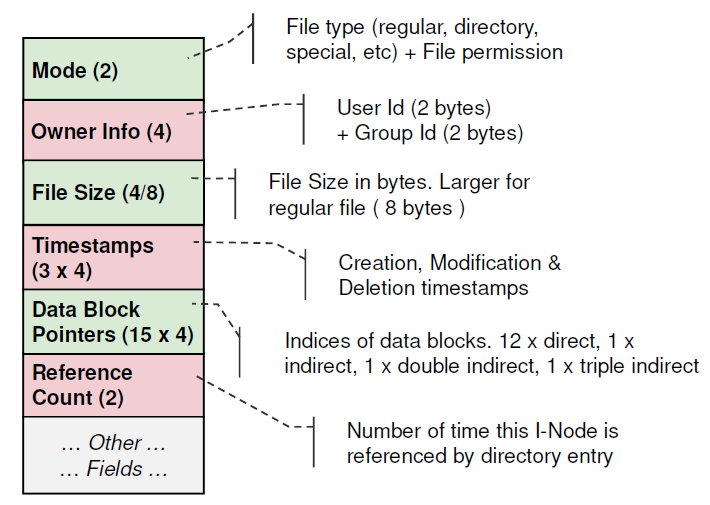
\includegraphics[width=0.4\textwidth]{12_3.png}
\end{figure}
Above is the I-Node Structure, which has size of 128 bytes.\\
For the data blocks of a directory, it stores a linked list of directory entries for file/subdirectories information within the directory. Each directory entry contains:
\begin{itemize}
  \item I-node number for that file/subdirectory
  \item Size of the directory entry, for locating the next directory entry
  \item Length of the file/subdirectory name
  \item Type; File or subdirectory
  \item File/Subdirectory name(up to 255 hracters)
\end{itemize}
It links to a $0$ I-node number to indicate unused entry.\\
Given a pathname, say \texttt{/sub/file}, let \texttt{currDir}=``/''. Root directory has a fixed I-node number $2$.\\
We read the actual I-node and check whether \texttt{sub} is a directory or file. If it is the direcotry, retrieve the I-node number and read the actual I-node. Otherwise, locate the directory entry in \texttt{CurrDir}, retreive I-node number and read actual I-node.\\

To delete a file, remove its directory entry rom parent directory. Point the previous entry to next entry/end.\\
We then update I-node bitmap, by marking corresponding I-node as free. Then we update block bitmap, by mark the corresponding block as free.\\

For sharing with hard/symbolic link, if it is a hard link, we create a directory entry in $B$ which uses the same I-node number. For symbolic link, creates a new file $Y$ in $B$ where $Y$ contains the pathname of $X$.
\end{document}
